\documentclass[envcountsect,runningheads]{llncs}
%
\usepackage{graphicx}
\usepackage{amsmath,amssymb,amscd,amstext}
\usepackage[utf8]{inputenc}
\makeatletter
\newcommand{\@chapapp}{\relax}
\makeatother

\usepackage{pst-node}
\usepackage{tikz,pgf}
\usepackage{tikz-cd} 
\usepackage{pgfplots}
\usepackage{pgfplotstable}
\pgfplotsset{compat=newest}
\usetikzlibrary{spy,decorations.markings,decorations.text,arrows.meta,bending,3d,shapes.arrows,positioning,fit,backgrounds,fadings}
\let\clipbox\relax

\usepackage{adjustbox}
\usepackage{mathtools}
\usepackage{setspace}
\usepackage{xcolor}
\usepackage{mathrsfs}
\usepackage{multibib}
\usepackage{filecontents}
\usepackage{slashbox}
\usepackage{multirow}
\usepackage{booktabs}
\newcommand{\ra}[1]{\renewcommand{\arraystretch}{#1}}

\usepackage[hidelinks]{hyperref}
\hypersetup{
    pdftitle={Invertible Resnets up to Homology Equivalence for Connected Abelian Lie Groups},    % title
    pdfauthor={Luciano Melodia},     % author
    pdfsubject={Invertible Neural Nets up to Homology Equivalence},   % subject of the document
    pdfcreator={Luciano Melodia},   % creator of the document
    pdfproducer={Luciano Melodia},  % producer of the document
    pdfkeywords={Embedding Dimension} {Parametrization} {Persistent Homology} {Neural Nets} {Manifold Learning}, % list of keywords
    pdfnewwindow=true,
    colorlinks,
	citecolor=black,
	filecolor=black,
	linkcolor=black,
	urlcolor=blue
}


\newcites{main}{References}

\definecolor{blacky}{RGB}{26,26,29}
\definecolor{gray}{RGB}{78,78,80}
\definecolor{purpur}{RGB}{111,34,50}
\definecolor{brick}{RGB}{149,7,64}
\definecolor{fire}{RGB}{195,7,63}

\newcommand{\gradient}[0]{\noindent%
    
\begin{tikzpicture}
    \fill[brick, path fading=west, left color=fire, right color=brick] (0,1em) rectangle (1cm,1.5em);
    \end{tikzpicture}%
}

\tikzset{circle dotted/.style={dash pattern=on .05mm off 2mm, line cap=round}}

\let\definition\relax
\let\lemma\relax
\let\corollary\relax
\let\theorem\relax
\let\proposition\relax
\let\example\relax
\let\remark\relax

\spnewtheorem{definition}{Definition}[section]{\bfseries}{\rmfamily}
\spnewtheorem{example}{Example}[definition]{\itshape}{\rmfamily}
\spnewtheorem{theorem}{Theorem}[section]{\bfseries}{\rmfamily}
\spnewtheorem{proposition}{Proposition}[theorem]{\bfseries}{\rmfamily}
\spnewtheorem{propositionsec}{Proposition}[section]{\bfseries}{\rmfamily}
\spnewtheorem{lemma}{Lemma}[theorem]{\bfseries}{\rmfamily}
\spnewtheorem{corollary}{Corollary}[lemma]{\bfseries}{\rmfamily}
\spnewtheorem{remark}{Remark}[example]{\itshape}{\rmfamily}
\spnewtheorem{remarkdef}{Remark}[definition]{\itshape}{\rmfamily}
\spnewtheorem{remarklem}{Remark}[lemma]{\itshape}{\rmfamily}
\spnewtheorem{remarktheo}{Remark}[theorem]{\itshape}{\rmfamily}
\spnewtheorem{remarkprop}{Remark}[proposition]{\itshape}{\rmfamily}
\DeclareMathOperator{\Ima}{im}
\DeclareMathOperator{\rank}{rank}
% Used for displaying a sample figure. If possible, figure files should
% be included in EPS format.
%
% If you use the hyperref package, please uncomment the following line
% to display URLs in blue roman font according to Springer's eBook style:
\renewcommand{\qed}{\hfill$\square$}
\renewcommand\UrlFont{\color{blue}\rmfamily}
\newcommand{\interior}[1]{%
  {\kern0pt#1}^{\mathrm{o}}%
}

\tikzset{->-/.style={decoration={markings, mark=at position #1 with {\arrow[line width=1pt]{>}}},postaction={decorate}}}
\begin{document}
%
\title{Invertible Resnets up to Homology Equivalence for Connected Abelian Lie Groups}
%
\titlerunning{Invertible Resnets up to Homology Equivalence}
% If the paper title is too long for the running head, you can set
% an abbreviated paper title here
%
\author{Luciano Melodia\orcidID{0000-0002-7584-7287} \\
\and Richard Lenz\orcidID{0000-0003-1551-4824}}
%
\authorrunning{L. Melodia et al.}
% First names are abbreviated in the running head.
% If there are more than two authors, 'et al.' is used.
%
\institute{Chair of Computer Science 6\\
Friedrich-Alexander University Erlangen-Nürnberg\\
91058 Erlangen, Germany \\
\email{\{luciano.melodia,richard.lenz\}@fau.de}}
%
\maketitle              % typeset the header of the contribution
%
\begin{abstract}
Neural nets have been used in an elusive number of scientific disciplines. Nevertheless, their parameterization is largely unexplored. Dense nets are the coordinate transformations of a manifold from which the data is sampled. After processing through a layer, the representation of the original manifold may change. This is crucial for the preservation of its topological structure and should therefore be parameterized correctly. We discuss a method to determine the smallest topology preserving layer for an invertible residual net. We consider the data domain as abelian connected matrix group and observe that it is decomposable into $\mathbb{R}^p \times \mathbb {T}^q$. Persistent homology allows us to count its $k$-th homology groups. Using Künneth's theorem, we count the $k$-th Betti numbers. Since we know the embedding dimension of $\mathbb{R}^p$ and $\mathcal{S}^1$, we parameterize the bottleneck layer with the smallest possible matrix group, which can represent a manifold with those homology groups. Resnets guarantee smaller embeddings due to the dimension of their state space representation.

\keywords{Embedding Dimension \and Parametrization \and Persistent Homology \and Neural Nets \and Manifold Learning.}
\end{abstract}

\section{Motivation}
Neural nets and their underlying principles were studied from the perspective of differential and information geometry \citemain{YangA97}. The natural gradient descent turned out to be Fisher optimal \citemain{Amari1,Amari2}, in its interpretation as a walk on the hypersurface of a neural loss function. Local minima, maxima and saddle points on the hypersurface have always been a problem when training machine learning models. A critical point on this surface corresponding to the global minimum of a smaller model forms a local minimum or saddle point of a larger one \citemain{FukumizuA00}. In other words, the critical values of a function represented by a layer of $(n-1)$-perceptrons will result in many critical values of a layer of $n$-perceptrons.

The manifold of a dense neural net is in most cases Euclidean, but it is restricted by the loss function or the data manifold to certain matrix groups. A metric is required to describe the geometric properties of such a manifold. Recently \citemain{HauserR17}, the change of coordinate systems and the learned metric tensor of a Riemann manifold during back propagation of neural nets was formulated. Further, it has been shown that dense neural nets can't approximate all functions arbitrarily precisely \citemain{Johnson19}. In response to this result, neural nets with residual connections were examined. Resnets add the output of one layer to a deeper one and therefore bypass some of the layers in between. This type of neural net is an universal function approximator \citemain{LinJ18}. The depth of the net is a parameter depending on the moduli of continuity of a function to be approximated \citemain{LinJ18}. Such a residual layer defines a forward or backward difference operator on a partition of the layers. The state space dimension with residual connections is homeomorphic to $\mathbb{R}^{k \cdot n}$, where $n = \text{dim} \; M$ and $k$ is the number of times the difference operator was used \citemain{HauserGJR19}. Estimating simplicial homology in connection with Künneth's theorem we found a resnet with an approximate minimal number of perceptrons for a very special learning problem.

We use invertible architectures, to demonstrate our hypothesis on a different Lie group from Euclidean space \citemain{NguyenAK19}. Our interpretation of a neural net is a continuous transformation, transferring invariant structures of the data in the input space to its deepest layer. Thus, it is capable to reconstruct the structure of the original space. This approach corresponds to the concept of homotopy equivalence \citemain{RubinsteinR08,YangY93}, which means that there is a continuous map $f: X \rightarrow Y$ and $g: Y \rightarrow X$, such that $f \circ g$ is homotopic to the identity $\text{Id}_Y$ and $g \circ f$ to $\text{Id}_X$. Thus, the spaces can be deformed continuously into one another. To do so, their homotopy groups must be equal. The fundamental group gives information about connected components which can be collapsed to a point by continuous functions, the first homotopy group about `holes' and the second about `cavities' and so forth. But homotopies are difficult to compute \citemain{klaus2004quick,hatcher2002algebraic}. Homology theory gives a remedy that guarantees an isomorphism between homotopy groups and homology groups under the conditions of Hurewicz's Theorem \citemain{klaus2004quick}. We use theoretical results from Lie theory and persistent homology theory to estimate how many dimensions of embedding are needed to represent the homology groups. Our paper is structured as follows:
\begin{itemize}
    \item In Sect. \ref{sec:manifoldassumption} we discuss the mathematical assumptions and recall the principles of smooth manifolds and Lie theory. In particular, we recall the decomposition of connected commutative Lie groups into $\mathbb{R}^p \times \mathbb{T}^q$.
    \item In Sect. \ref{sec:persistenthomology} we introduce to the theory of persistent homology, define persistence diagrams, persistence landscapes and confidence sets, in order to estimate homology groups despite noisy data. We use Künneth's theorem and derive how to count the homology groups of the input space.
    \item In Sect. \ref{sec:neuralnettheory} we explain the mathematical theory of neural nets and construct invertible deep neural nets to satisfy our assumptions. Resnets, which have a larger state space dimension, offer an architecture with a comparatively small number of parameters to dense nets.
    \item In Sect. \ref{sec:numericalexperiments} we validate our theory training autoencoders on the cifar10 and cifar100 datasets, isolating the innermost layer such that no residual connections bypass it on different embedding dimensions.
\end{itemize}

\section{The Manifold Assumption}
\label{sec:manifoldassumption}
The manifold assumption states that a point $x = \{x_1, \cdots, x_d\} \in \mathbb{R}^n$ lies on an embedded manifold $M$, with $\dim M \ll n$. We specify the concept of smooth manifolds. Then we dive into Lie groups concluding with a central theorem on the isomorphism of abelian connected Lie groups to the product space $\mathbb{R}^p \times \mathbb{T}^q$, which turns out useful to estimate the embedding dimension of the manifold.

\subsection{Background: Smooth Manifolds}
Manifolds generalize the concept of space mathematically. They are described by a collection of local coordinate maps $\varphi: U \rightarrow \varphi(U) \subseteq \mathbb{R}^n$ which are homeomorphic to $\mathbb{R}^{n}$ where $n = \text{dim} \; M$ and an open neighborhood $(U_i,\varphi_i)$ in $M$ which is covered by this map. The union of such maps should cover the entire space, i.e. $M = \bigcup_{i \in I} U_i$ and is called \textit{atlas} $\mathcal{A} = \{(U_i,\varphi_i) \; \vert \; i \in I\}$ \citemain{lee2013smooth}. The functions $x_1, \cdots, x_n: U \rightarrow \mathbb{R}$ are called local coordinates $\varphi(p) = (x_1(p), \cdots, x_n(p))$. 

We require that the coordinate system on $M$ is smooth. This is due to the condition that two maps of a differentiable structure must always be compatible with each other. Compatibility means, that the maps $(U,\varphi), (V,\psi)$ are diffeomorphic, such that their composition $\psi \circ \varphi^{-1}:\varphi(U \cap V) \rightarrow \psi(U \cap V)$ is a diffeomorphism between the two open subsets $\varphi(U \cap V)$, $\psi(U \cap V) \subseteq \mathbb{R}^n$, i.e. $\psi \circ \varphi^{-1}$ and $\varphi \circ \psi^{-1}$ are in $\mathcal{C}^\infty(M)$. Therefore, they are also smooth. If we take a step back and neglect smoothness for $M$, then $M$ is a topological manifold. 

If we now equip $M$ with such an atlas $\mathcal{A}$ and if this atlas is maximal with respect to inclusion, then it is a \emph{differentiable structure}. Each atlas for $M$ is included in a maximal atlas. Because of the differentiable structure, the maps in $\mathcal{A}$ are also compatible with all other maps of $\mathcal{A}_{max}$ \citemain{lee2013smooth}. Thus, it is sufficient to describe smooth manifolds by an atlas that is not maximal.

\subsection{Background: Lie groups}
\label{liegroups}
A Lie group is a $\mathcal{C}^\infty$-manifold $G$ which is equipped with a group structure such that the maps $\mu:(x,y) \mapsto xy, G \times G \rightarrow G$ and $\imath: x \mapsto x^{-1}, G \rightarrow G$ are smooth. In our case $\mu$ corresponds to the matrix multiplication. The neutral element of a group is denoted by $e = e_G$. Each abelian commutative Lie group $G$ of dimension $\dim G = m$ is isomorphic to a particular product space $\mathbb{R}^p \times \mathbb{T}^q$, with $p + q = m$, see Appx. \ref{connectedcommutativeliegroupdecomposition}. Thus, the group can be decomposed into a product space with a relatively simple topological structure. The $q$-torus $\mathbb{T}^q$ is a surface of revolution. It moves a curve around an axis of rotation. These axes are given by $1$-spheres, so the $q$-torus is the product space $\mathbb{T}^q := \mathcal{S}^1_1 \times \cdots \times \mathcal{S}^1_q$. Our initial decomposition of the Lie group into a product space can be further simplified into $G \simeq \mathbb{R}^p \times (\mathcal{S}^1_1 \times \cdots \times \mathcal{S}^1_q)$. Note, that the $(n-1)$-sphere is given by $\mathcal{S}^{n-1} := \{x \in \mathbb{R}^n \; \vert \; ||x||_2 = 1\}$. Thus, $\mathcal{S}^1$ can be embedded into a two-dimensional Euclidean space. The homology groups and the embedding dimensions of the product spaces, yield by decomposition of connected commutative Lie groups, are therefore known. Any Euclidean space like $\mathbb{R}^p$ is contractible, i.e. zero-homotopic or homotopy equivalent to a constant map, thus the homology group $H_k(\mathbb{R}^p) = 0$ for $k > 0$ and $H_k(\mathbb{R}^p) = \mathbb{Z}$ for $k = 0$. To illustrate the role of orientation, we calculate the homology groups and illustrate the triangulation of the $1$-sphere, both with coefficients in $\mathbb{R}$ and in $\mathbb{Z}/2\mathbb{Z}$ in Fig. \ref{complexes}. The latter field neglects orientation. Note, that for this field $+1 = -1$.

A tool is needed to estimate homology groups of the manifold on which the data points lie. The method can then be inversely applied to the homology groups to estimate its embedding dimension. We introduce persistent homology with its confidence intervals in order to obtain the best possible estimate of the current state of the art by removing topological noise.

\section{Persistent Homology}
\label{sec:persistenthomology}
In algebraic topology spaces are studied as the composition of triangles, the latter being used as the fundamental component of a large class of spaces. All closed surfaces can be constructed by identifying -- or, less formally, `gluing' -- the edges of triangles \citemain[p.~102]{hatcher2002algebraic,lume}. The $n$-dimensional generalization of triangles are $n$-\emph{simplices}. They are the smallest convex set in Euclidean space with $(n+1)$-points $v_0,\cdots,v_n$, which have no solutions for any system of linear equations in $n$-variables. Thus, they do not lie on any hyperplane with a dimension less than $n$ \citemain[p.~103]{hatcher2002algebraic}. We define the $n$-simplex as follows:
\begin{equation}
    \Delta^n = \left\{ [v_0,\cdots,v_n] \in \mathbb{R}^{n+1} \; \bigg\vert \; \sum_{i=0}^{n} v_i = 1 \; \text{and} \; v_i \geq 0 \; \text{for all} \; i \right\}.
\end{equation}
Removing a vertex from $\Delta^n$ results in a $(n-1)$-simplex called \emph{face} of $\Delta^n$. The combinatorial description of $n$-simplices is called \emph{simplicial complex}.

\subsection{Simplicial Complexes and Homology Theory}
\label{simcomplexhomtheory}
Simplicial homology is studied by $\Delta$-complexes whose simplices are uniquely determined by their vertices. Thus, every $n$-simplex has $(n+1)$ distinct vertices and no other $n$-simplex has the same set of vertices. A \emph{simplicial complex} $K$ is a collection of simplices, such that any face of a simplex of $K$ is a simplex of $K$ and the intersection of any two simplices of $K$ is either empty or a common face of both \cite[p.~11]{boissonnat2018geometric}. This is a unique combinatorial description of vertices together with a collection of sets $\{\Delta^k_1, \cdots, \Delta^k_m\}$ of $k$-simplices, which are $(k+1)$ element subsets of $K$ \citemain[p.~107]{hatcher2002algebraic}. Further, we require every $(k+1)$-element, with $k < n$ to be a $k$-simplex of $\Delta^k \subset K$. Simplicial complexes have a natural order of simplices, which is illustrated in Fig. \ref{complexes}. It plays a central role in their geometric realization \citemain[p.~14]{boissonnat2018geometric}. If we choose a total order for all corners which are located in any simplex of $K$, we get an order for each single $k$-simplex.

A \textit{singular $k$-simplex} is defined as a continuous map $\sigma: \Delta^k \rightarrow X$ into a topological space $X$. Intuitively, every simplicial complex $K$ has some connected components. These form a vector space $C_k(X)$, which is called \textit{$k$-th chain group}, with coefficients in $\mathbb{Z}$ and elements called $k$-\textit{chains}. The $k$-chains are finite sums $\sum_{i=0}^{k} z_i \sigma_i$ with $z_i \in \mathbb{Z}$ \citemain[p.~108]{hatcher2002algebraic}. Having connected components defined as a group implies also the definition of a boundary. As the boundaries of a $k$-simplex are also $(k-1)$-simplices, we can remove all other simplices to project into the lower chain group by the $k$-th boundary operator $\partial_k: C_k(X) \rightarrow C_{k-1}(X)$:
\begin{equation}
    \partial_k(\sigma) = \sum_{i=0}^{k} (-1)^{i} \sigma \bigg\vert {[v_0,\cdots,\hat{v}_i, \cdots, v_k]}.
\end{equation}
Observe that the composition of boundary maps is zero, as a boundary has no boundary by itself, i.e. $\partial_i\partial_{i+1} = 0$ \citemain[pp.~108--109]{hatcher2002algebraic}. Thus, $\ker \; \partial_i$ corresponds to the generating elements of the $i$-th boundary group and $\Ima \; \partial_{i+1}$ for the $i$-th chain group. The singular homology group is the quotient space
\begin{equation}
    H_k(X) = \frac{\ker \left(\partial_k: C_k\left(X\right) \rightarrow C_{k-1}\left(X\right)\right)}{\Ima \left(\partial_{k+1}:C_{k+1}\left(X\right) \rightarrow C_{k}\left(X\right)\right)}.
\end{equation}
The $k$-th singular homology group is isomorphic to the $k$-th simplicial homology group for a trianguliable metric space, i.e. $H_k(X) \simeq H^{\Delta}_k(X)$ for all $k \in \mathbb{Z}$, see Appx. \ref{simplicialsingularequivalence}, thus we can transfer results from one homology theory to the other.

Examining the homology groups of a set of points gives us little information about the structure of our dataset. However, since the homology groups of a simplicial complex are equal to the direct sum of the ones of all disjoint subcomplexes, see Appx. \ref{directsums}, we examine them more closely. In particular, we are interested in a parametrization of the simplicial complex as geometric realization in which the homology groups appear and disappear again. For this purpose we consider all possible subcomplexes that form a \emph{filtration} over the point cloud $X$. Depending on how we vary the parameter $\omega_i$ of the chosen simplicial complex, the following sequence is generated, starting with the empty set:
\begin{align}
	\emptyset &= K^{\omega_0}(X) \subset K^{\omega_1}(X) \subset \cdots \subset K^{\omega_{n+1}}(X) = K(X),\\
	K^{\omega_{i+1}}(X) &= K^{\omega_i}(X) \cup \sigma^{\omega_{i+1}}, \quad \text{for} \; i \in \{0, \cdots, n-1\}.
\end{align}
The filtration has a discrete realization with a fixed $\epsilon = \omega_{i+1}-\omega_{i} = \min(x,y)$ for all $x,y \in X$. We chose a sufficiently small $\epsilon$, in order to capture the birth and death of critical values in the sublevel sets of the simplicial complex upon the data, to be able to map as much structure as possible into the persistence diagram -- which clearly depends on the metric.
\begin{figure}[t]
    \begin{overpic}[width=\textwidth,tics=10]{figure1.pdf}
        \put (0.9,58) {\textbf{a})}
        \put (0.9,28) {\textbf{b})}
        \put (70,58) {\textbf{c})}
        \put (8.8,29.6) {$0$}
        \put (32.8,29.6) {$0$}
        \put (58,29.6) {$0$}
        \put (74.8,43.6) {\small{1}}
        \put (90.5,43.6) {\small{2}}
        \put (84.6,22.4) {\small{3}}
        \put (84.6,1) {\small{4}}
        \put (7,13) {$K_1$}
        \put (31,13) {$K_2$}
        \put (57,13) {$K_3$}
        \put (21,13) {$\subseteq$}
        \put (45,13) {$\subseteq$}
        \put (32,39) {$B_k$}
        \put (32,49) {$Z_k$}
        \put (32,55) {$C_k$}
        \put (56,39) {$B_{k-1}$}
        \put (56,49) {$Z_{k-1}$}
        \put (56,55) {$C_{k-1}$}
        \put (7,39) {$B_{k+1}$}
        \put (7,49) {$Z_{k+1}$}
        \put (7,55) {$C_{k+1}$}
        \put (19.5,56) {$\partial_{k+1}$}
        \put (44.5,56) {$\partial_{k}$}
        \put (92,37) {{\color{red5} $\bullet$} $H_0$}
        \put (92,34) {{\color{red4} $\bullet$} $H_1$}
        \put (92,31) {{\color{red3} $\bullet$} $H_2$}
        \put (92,28) {{\color{red2} $\bullet$} $H_3$}
        \put (92,25) {$\cdots$}
        \put (92,15.5) {{\color{red5} $\bullet$} $H_0$}
        \put (92,12.5) {{\color{red4} $\bullet$} $H_1$}
        \put (92,9.5) {{\color{red3} $\bullet$} $H_2$}
        \put (92,6.5) {{\color{red2} $\bullet$} $H_3$}
        \put (92,3.5) {$\cdots$}
    \end{overpic}\\[0.1cm]
    \caption{\textbf{a}) Illustration of the chain complex following Zomorodian et al. \cite{ZomorodianC05}. \textbf{b}) Sublevel sets of a simplicial complex connected by inclusion. \textbf{c}) Pipeline for persistent homology: \textbf{c})1. Loading point sets. \textbf{c})2. Computation of a filtration. \textbf{c})3. Computation of persistent homology with confidence band. \textbf{c})4. Computation of persistence landscapes.}
    \label{figure1}
\end{figure}


\subsection{Persistence Diagrams}
Recording the \emph{Betti numbers} of the $k$-th homology group along the filtration, we obtain the \emph{$k$-dimensional persistence diagram}. The Betti numbers $\beta_k$ are defined by $\rank(H_k(X))$. We write $H^{\omega_i}_k = H_k(K^{\omega_i}(X))$ as $k$-th homology group on the simplicial complex $K$ with parametrization $\omega_i$. Then $H^{\omega_{i}}_{k} \rightarrow H^{\omega_{i+1}}_k$ induces a sequence of homomorphisms on the filtration, see Appx. \ref{persistenthomologyproofs} \citemain{lume,edelsbrunner2008persistent}:
\begin{align}
0 = H^{\omega_{0}}_k \rightarrow H^{\omega_{1}}_k \rightarrow \cdots \rightarrow H^{\omega_{n}}_k \rightarrow H^{\omega_{n+1}}_k = 0.
\end{align}
The image of each homomorphism consists of all $k$-dimensional homology classes which are born in $K^{\omega_i}(X)$ or appear before and die after spanning $K^{\omega_{i+1}}(X)$. Tracking the Betti numbers on the filtration results into a multiplicity
\begin{equation}
\mu^{\omega_{i},\omega_{j}}_k := (\beta_k^{\omega_{i},\omega_{j-1}} - \beta_k^{\omega_i,\omega_{j}})-(\beta_k^{\omega_{i-1},\omega_{j-1}}-\beta_k^{\omega_{i-1},\omega_{j}})
\end{equation}
for the $k$-th homology group and index pairs $(\omega_i,\omega_{j+1}) \in \overline{\mathbb{R}^2} := \mathbb{R}^2 \cup \infty$ with indices $i \leq j$ \citemain{edelsbrunner2008persistent}. The Euclidean space is extended, as the first connected component of our filtration is not merged with any other critical value. We assign the value $\infty$ to it, corresponding to the second coordinate $w_{j+1}$ in the persistence diagram. The first term counts elements born in $K^{\omega_{j-1}}(X)$ and vanished entering $K^{\omega_{j}}(X)$, while the second term counts the representatives of homology classes before $K^{\omega_{j}}(X)$ and vanishing at $K^{\omega_{j}}(X)$. The index pairs denote the \emph{birth} and \emph{death} of a homology class. The $k$-th persistence diagram is thus
\begin{equation}
\mathfrak{P}_k(K(X)) := \left\{(\omega_i, \omega_{j+1}) \in \overline{\mathbb{R}^2} \; \bigg\vert \; \mu^{\omega_{i},\omega_{j+1}}_k = 1 \; \text{for all} \; i,j \in I \right\}.
\end{equation}

\subsection{Confidence Sets}
We are interested in the homology groups of $M$ and not in those of $K(X)$. Nevertheless, the point set $X$ is drawn from a distribution, that is either on or near $M \subset \mathbb{R}^d$. We need to decide whether a persistent homology class comes from this distribution or not. For this purpose, confidence intervals for persistence diagrams have been defined \citemain{bubenik2015statistical,fasy2014confidence}. A confidence interval starts at the off-diagonal of a persistence diagram and ends parallel to it. It determines which topological features are persistent enough, i.e. persist in the filtration long enough to be recognized as such. Otherwise, they are treated as topological noise and removed.

For two compact sets $X,Y \subset \mathbb{R}^n$, the persistent homology on their filtration is stable with respect to the Hausdorff distance \citemain{fasy2014confidence}, which is defined as
\begin{align}
d_H(X,Y) := \max\left\{\sup_{x \in X} \inf_{y \in Y} d(x,y), \sup_{y \in Y} \inf_{x \in X} d(x,y) \right\}.
\end{align}
Furthermore, persistent homology is stable with respect to the bottleneck distance -- an extremal case of the Wasserstein distance -- for some $p \rightarrow \infty$:
\begin{align}
d_B(X,Y) := \inf_{\varphi: X \rightarrow Y} \sup_{x \in X} ||x-\varphi(x)||_p,
\end{align}
with $\varphi$ beeing within the set of all bijections from $X$ into $Y$, yielding
\begin{align}
	d_B\left(\mathfrak{P}\left(K\left(X\right)\right), \mathfrak{P}\left(K\left(Y\right)\right)\right) \leq c \cdot d_H\left(X,Y\right).
\end{align}
Let $\mathbb{P}$ be a distribution of a finite set of points $X$ and $x \in X$ a sample drawn from this distribution. Then we can define a confidence interval with respect to the Hausdorff distance as $\mathbb{P}\left( d_H(x,X) \leq \mu_\alpha \right) \geq 1-\alpha$ \citemain{fasy2014confidence}. A persistence confidence set $\mathscr{C}(K(X))$ is a subset of all persistence diagrams which have a certain distance from the diagonal. We look for all homology classes persisting a minimum `time':
\begin{align}
	\mathscr{C}(K(X)) := \left\{ \mathfrak{P}(K(X)) \; \bigg\vert \; c \cdot d_B\left(\text{Diag}\left(\mathfrak{P}\left(K\left(X\right)\right)\right), \mathfrak{P}\left(K\left(X\right)\right) \right) \leq \mu_\alpha \right\}.
\end{align}
Recall, that no points can appear under the diagonal line. Therefore, we measure the distance to the diagonal. For $d_B(x,y)$ imagine a box around each point with a certain radius $\mu$. If the diagonal of the persistence diagram passes through the box of a point, the point is considered as noise and removed.

\subsection{Persistence Landscapes}
The summaries of topologically persistent features -- with the purpose of computing statistics in a Hilbert space -- was initiated by Bubenik \citemain{bubenik2015statistical}. Bubenik and Dlotko first provided efficient algorithms to compute persistence landscapes \citemain{bubenikD17}. Persistence landscapes give a summary of the topology of a set of points embedded in a given topological manifold. Looking at the points $(\omega_i,\omega_{j+1}) \in \overline{\mathbb{R}^2}$ on the $k$-th persistence diagram $\mathfrak{P}_k(K(X))$, one associates a piecewise linear function $f_{(\omega_i,\omega_{j+1})}: \mathbb{R} \rightarrow [0,\infty)$ with them, which is defined as
\[
    f_{(\omega_i,\omega_{j+1})}(x) =
\begin{dcases}
    0,
    & \text{if} \; x \not\in (\omega_i,\omega_{j+1}),\\
    x - \omega_{i},
    & \text{if} \; x \in \left(\omega_{i},\frac{\omega_i + \omega_{j+1}}{2} \right],\\
    \omega_{j+1} - x 
    & \text{if} \; x \in \left(\frac{\omega_i + \omega_{j+1}}{2},\omega_{j+1} \right).
\end{dcases}
\]
We describe the summaries for the general persistence diagram, beeing the disjoint union of the $k$-th persistence diagrams $\mathfrak{P}(K(X)) := \coprod_{i=0}^{k} \mathfrak{P}_i(K(X))$. A persistence landscape $\mathfrak{L}(\mathfrak{P}(K(X)))$, contains the birth-death pairs $(\omega_i,\omega_{j+1})$, for an $i,j \in \{1, \cdots, n\}$ and is the function sequence $\lambda_k : \mathbb{R} \rightarrow [0,\infty)$ for a $k \in \mathbb{N}$, where $\lambda_k(x)$ denotes the $k$-th greatest value of $f_{(\omega_i,\omega_{j+1})}(x)$. Thus, $\lambda_k(x) = 0$ if $k > n$. In contrast to standard topological summaries, the persistence landscape lies in a completely normed vector space, suited for statistical computations.

\subsection{Counting Betti Numbers}
In the following, the homology groups are computed over $\mathbb{Z}$. Based on our assumption to operate on a connected commutative Lie group, there is an isomorphism for the homology groups of the data space $G$, so that $H_k(G) \simeq H_k(\mathbb{R}^p \times \mathcal{S}^{1}_{1}\times\cdots\times\mathcal{S}^{1}_{q})$ with $p+q = \dim G$, see \ref{decomposition}. The homology groups of this product space are equal to the homology groups of the sought manifold. The neural net should be able to preserve all structures within this space. Since the input domain is a set of points to be described by one or more compact manifolds, all homology classes should be preserved in our learning task. Künneth's theorem states that the $k$-th singular homology group of a topological product space $X \times Y$ is isomorphic to the product of the respective $k$-th homology groups of $X$ and $Y$, see \citemain[p.~268]{hatcher2002algebraic} and Appx. \ref{a:groups}:
\begin{align}
    H_k(X \times Y) \simeq \bigoplus_{i+j=k}H_i(X) \otimes H_j(Y).
\end{align}
This applies to all fields, since modules over a field are always free. If we apply the theorem to the decomposition, we get for the space we are looking for
\begin{align}
	\label{homologykunneth}
    &H_k(\mathcal{S}^{1}_{1}\times\cdots\times \mathcal{S}^{1}_{q}\times\mathbb{R}^p) \simeq \\
    \simeq \bigoplus_{i_{1} + \cdots + i_{r}=k} &H_{i_{1}}(\mathcal{S}^{1}_{1}) \otimes \cdots \otimes H_{i_{\hat{r}}}(\mathcal{S}^{1}_{q}) \otimes H_{i_{r}}(\mathbb{R}^{p}).
\end{align}
We need to know how to count in order to derive the dimension of the sought manifold from the representatives of homology classes within the mean persistence landscapes. Note, in Eq. \ref{homologykunneth} terms remain only for indices $i_{j} \in \{0,1\}$. Thus, the homology group $H_k(\mathbb{T}^{q}) \simeq H_k(\mathcal{S}^{1}_{1} \times \cdots \times \mathcal{S}^{1}_{q}) \simeq \mathbb{Z}^{{q\choose{k}}}$ and $H_0(\mathbb{R}^p)\simeq\mathbb{Z}^{p}$, where $p$ indicates the number of connected components. We denote the amount of representatives from homology classes of the $k$-th homology group appearing in the mean persistence landscape $\bar{\mathfrak{L}}$ by $\sharp^{H}_{k}(\bar{\mathfrak{L}}(\mathfrak{P}(K(X)))$. Thus, we get the following relation for the representatives of the zeroth homology group:
\begin{align}
	\label{countingsimple}
	\sharp_{0}^{H}(\bar{\mathfrak{L}}(K(X))) \approx p.
\end{align}
This is the number of connected components to be represented by the innermost layer of the neural net, corresponding exactly to the number of elements from the zeroth homology group. We only need to consider the homology groups which are represented in the mean persistence landscape. Assuming that our estimate is good, higher homology groups are trivial. The required number of factors of $1$-spheres can be determined for the $k$-th homology group by
\begin{align}
	\label{countingequation}
	\sharp_{k}^{H}(\bar{\mathfrak{L}}(\mathfrak{P}(K(X))) \approx \prod_{i=1}^{k} \frac{q-k+i}{i}.
\end{align}
Note, that we assume to work on a smooth manifold, whose de Rham cohomology induces an isomorphism into the simplicial homology with coefficients in $\mathbb{R}$, see Appx. \ref{simplicialsingularequivalence}. We can still work with coefficients in $\mathbb{Z}$ because, according to the Universal Coefficient Theorem, the integral homology groups determine the homology groups over every field \cite{gruenberg1968universal}. Thus, these results can be applied without restriction to any homology theory, see Appx. \ref{simplicialsingularequivalence}.

\section{Neural Nets}
\label{sec:neuralnettheory}
Neural nets are a composition of affine transformations with a non-linear activation function. The projection on the $(l+1)$-th layer can be formalized as
\begin{equation}
\label{neuralnet}
    \varphi^{(l+1)} := \textbf{x}^{(l+1)} = \sigma(\mathbf{W}^{(l+1)} \cdot \textbf{x}^{(l)}+\textbf{b}^{(l+1)}).
\end{equation}
The linear map $\textbf{x} \mapsto \mathbf{W} \textbf{x}$ and the statistical distortion term $\textbf{x} \mapsto \textbf{x}+\textbf{b}$ is determined by stochastic gradient descent.  Note, that the linear transformation $\textbf{x} \mapsto \mathbf{W} \cdot \textbf{x}$ is interpreted as the product of a matrix $\mathbf{W}_{ij} = \mathbf{\delta}_{ij}\mathbf{W}_i$ with the input vector $\textbf{x}$ and the Kronecker delta, while $(\cdot)$ denotes elementwise multiplication.

$\sigma$ denotes a non-linear activation function. Commonly used are functions from the exponential family. A feedforward net is then a map $\varphi^{(l)}:\textbf{x}^{(l)}(M)$ $\rightarrow$ $\left(\varphi^{(l)}\circ \textbf{x}^{(l)}\right)(M)$. $\textbf{x}^{(0)} \in M$ are points on a Riemann manifold $M$. Learning by back propagation can be considered as a change of coordinate representation or shift on the tangent bundle of the underlying manifold \citemain{rumelhart1986learning}.

\subsection{Deep Learning}
\begin{figure}[t!]
\centering
\begin{tikzpicture}
\begin{axis}[
	height=2.2in,
	width= 2.6in,
	axis x line = bottom,
	axis y line = left,
	minor x tick num=10,
	ylabel={$\frac{\epsilon_i + \epsilon_{j+1}}{2}$},
	xlabel={\textbf{a}) Persistence landscape \texttt{cifar10}.},
	xmin=0,
	xmax=1050,
	ymin=0,
	ymax=650,
	ticklabel style={font=\small},
	x label style={at={(axis description cs:0.5,-0.1)},anchor=north},
	y label style={at={(axis description cs:0.20,0.85)},rotate=-90,anchor=south, fill=white},
	axis line style={-{Latex[length=1.5mm,width=1.5mm]}}
]
\coordinate (spypoint) at (axis cs:88,50);
\coordinate (magnifyglass) at (axis cs:800,400);
\draw [thick, dotted, draw=gray] (axis cs: 0,580) -- (axis cs: 1050,580) node[pos=0.9, below] {$\infty$};
\end{axis}
\begin{scope}[spy using outlines={circle, magnification=4, connect spies}]
\node[inner sep=0pt] at (2.38,1.77) {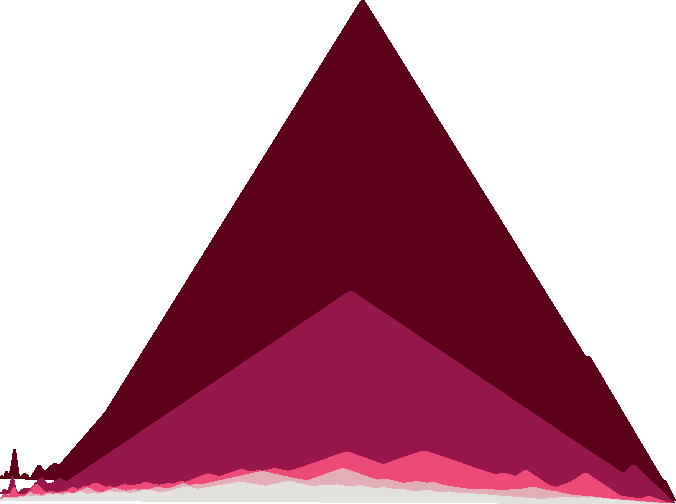
\includegraphics[width=0.39\textwidth]{figure2_a.pdf}};
\spy [lightgray, size=2cm] on (spypoint) in node[fill=white] at (magnifyglass);
\end{scope} 
\end{tikzpicture}
\begin{tikzpicture}
\begin{axis}[
	height=2.2in,
	width= 2.6in,
	axis x line = bottom,
	axis y line = left,
	minor x tick num=10,
	xlabel={\textbf{b}) Persistence landscape \texttt{cifar100}.},
	xmin=0,
	xmax=1050,
	ylabel={$\cdot 10^{3}$},
	ymin=0,
	ymax=5,
	ticklabel style={font=\small, fill=white},
	x label style={at={(axis description cs:0.5,-0.1)},anchor=north},
	y label style={at={(axis description cs:0.1,0.9)},rotate=-90,anchor=south},
	axis line style={-{Latex[length=1.5mm,width=1.5mm]}}
]
\draw [thick, dotted, draw=gray] (axis cs: 0,4.45) -- (axis cs: 1050,4.45) node[pos=0.9, below] {$\infty$};
\end{axis}
\node[inner sep=0pt] (h) at (2.38,1.77) {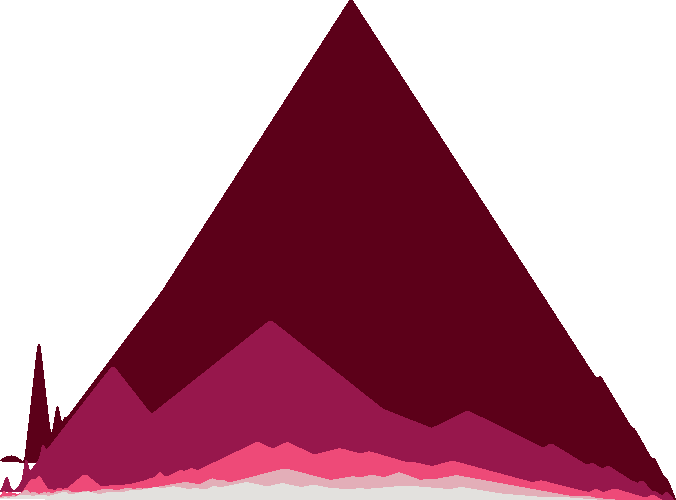
\includegraphics[width=0.39\textwidth]{figure2_b.pdf}};
\node[inner sep=0pt] (h) at (4.5,2.7) {{\color{red5}$\bullet$} {$H_0$}};
\node[inner sep=0pt] (h) at (4.5,2.3) {{\color{red4}$\bullet$} {$H_1$}};
\node[inner sep=0pt] (h) at (4.5,1.9) {{\color{red3}$\bullet$} {$H_2$}};
\node[inner sep=0pt] (h) at (4.5,1.5) {{\color{red2}$\bullet$} {$H_3$}};
\node[inner sep=0pt] (h) at (4.5,1.1) {{\color{red1}$\bullet$} {$H_4$}};
\end{tikzpicture}
\begin{tikzpicture}
	\begin{axis}[
	table/col sep=comma,
	xlabel={\textbf{c}) Validation loss \texttt{cifar10}.},
	height=2.2in,
	width= 2.6in,
   	ticklabel style={font=\small, fill=white},
	xticklabel style={rotate=90, anchor=near xticklabel},
	x label style={at={(axis description cs:0.5,-0.15)},anchor=north},
	xtick={0,0.1,0.2,0.4,0.6,0.8,1},
    xticklabels={dummy,0,50,100,150,200,250},
	]
	\end{axis}
	\node[inner sep=0pt] at (2.51,2.08) {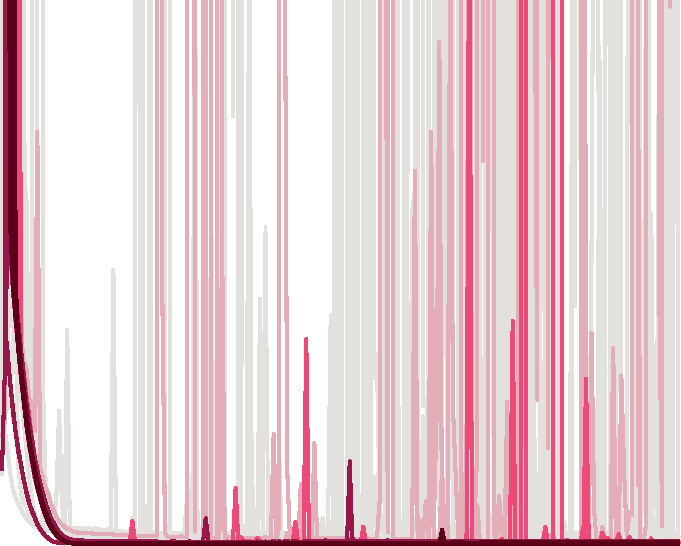
\includegraphics[width=0.343\textwidth, height=3.84cm]{figure2_c.pdf}};
\end{tikzpicture}
\begin{tikzpicture}
	\begin{axis}[
	table/col sep=comma,
	xlabel={\textbf{d}) Validation loss \texttt{cifar100}.},
	height=2.2in,
	width= 2.6in,
	ticklabel style={font=\small, fill=white},
	xticklabel style={rotate=90, anchor=near xticklabel},
	x label style={at={(axis description cs:0.5,-0.15)},anchor=north},
	xtick={0,0.1,0.2,0.4,0.6,0.8,1},
    xticklabels={dummy,0,50,100,150,200,250},
	]
	\end{axis}
	\node[inner sep=0pt] at (2.51,2.08) {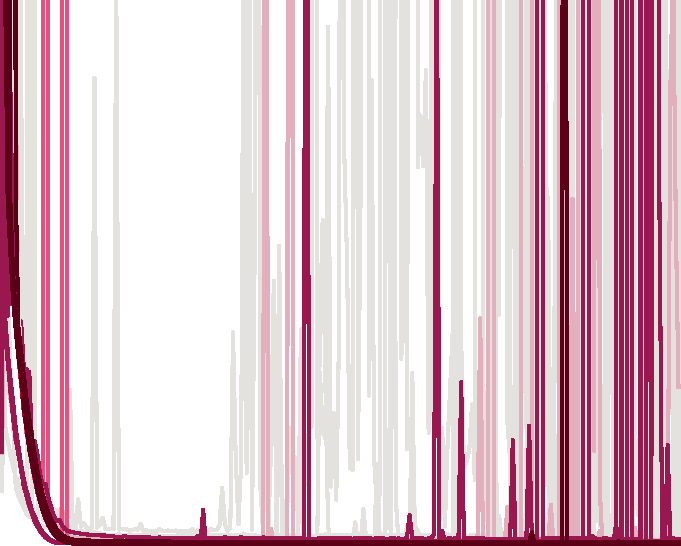
\includegraphics[width=0.343\textwidth, height=3.84cm]{figure2_d.pdf}};
\end{tikzpicture}
\caption{a) Persistence landscape for \texttt{cifar10} and b) for the \texttt{cifar100} dataset \cite{krizhevsky2009learning}. Persistence landscapes are computed up to a resolution of $10^3$. c) and d) show the \texttt{MSE} loss function on the validation dataset using a $7:3$ split.}
\label{figure2}
\end{figure}
Neural nets are used in practice with a different number of perceptrons per layer. However, a layer, from the perspective of a matrix group, can also represent the manifold of the previous one. Manifolds can always be immersed and submersed as long as the rank of the Jacobian of the respective map remains constant. Thus, the dimension of the data manifold is the dimension of the smallest possible bottleneck layer of the neural net  $\dim M = \min_l \dim \textbf{x}^{(l)}$ \citemain{HauserR17}. Our contribution provides the theory of how this dimension can be determined for all neural nets that are a composition of invertible layers acting on an abelian Lie group as domain of the data. The concatenation of such maps is called a deep neural net:
\begin{equation}
    \textbf{x}^{(L)}(M) = \left(\varphi^{(l+1)} \circ \varphi^{(l)} \cdots \circ \varphi^{(1)} \circ \varphi^{(0)} \circ \textbf{x}^{(0)}\right)(M).
\end{equation}
Activation functions restrict to a subgroup of Euclidean space. Continuous homomorphisms between Lie groups are automatically smooth. Thus, a second countable locally Euclidean group has exactly one differentiable structure, turning it into a Lie group. We need to show that $\textbf{x}^{(l+1)}$ has the topology of $G$ and is therefore an embedded closed Lie subgroup $\textbf{x}^{(l)} := H \subseteq G$. Cartans Theorem of Closed Subgroups states that a subgroup $H$ of a Lie group $G$ is an embedded Lie subgroup, if it is a closed subgroup \citemain{cartan1952theorie}. We construct our neural nets such that they are a subset of $\text{GL}(n,\mathbb{R})$ and according to the proof in Appx. \ref{liegroups}, this is a closed subgroup of $\text{GL}(n,\mathbb{C})$, which is itself a Lie group. It follows that a layer in the neural net is also a Lie group. Due to invertibility, the subsequent smaller layers are Lie subgroups, as $\sigma^{(l)}$ is smooth.

\subsection{Residual Neural Networks}
\label{resnet}
A \textit{resnet} skips some of the layers by adding outputs to a deeper layers. It has one \textit{skip connection} and is a $\mathcal{C}^1$-continuous dynamic transformation \citemain{he2016deep,HauserGJR19}:
\begin{align}
	\label{residualnet}
	\textbf{x}^{(l+1)} = \textbf{x}^{(l)} + \sigma^{(l)}\left(\textbf{x}^{(l)}\right) \Delta l.
\end{align}
The term $\Delta l$ in Eq. \ref{residualnet} is inserted as a perturbation term. In the work of Hauser et al. \citemain{HauserR17}, neural nets were classified as $\mathcal{C}^k$-architecture, depending on how often a \textit{finite difference operator} is applied to the map $\textbf{x}: M \times I \rightarrow \mathbb{R}^d$. The forward and backward difference operators are defined as $\delta^{+}: \textbf{x}^{(l)} \mapsto \textbf{x}^{(l+1)} - \textbf{x}^{(l)}$ and $\delta^{-}: \textbf{x}^{(l)} \mapsto \textbf{x}^{(l)} - \textbf{x}^{(l-1)}$. In this theory, we can write the difference operators for a general $n \in \mathbb{N}$ with explicit specification of the perturbation $\Delta l$ as
\begin{align}
	\label{generalresidual}
	\delta^+\left( \delta^- \right)^{n-1} \textbf{x}^{(l)} = \sum_{l'=0}^{k} \left[ (-1)^{l'} {k \choose l'} \textbf{x}^{(l+1-l')} \right] = \sigma^{(l)} \left(\textbf{x}^{(l)}\right) \Delta l^k.
\end{align}
We use the same notation as in \citemain{HauserGJR19}, where $(\delta^-)^{k-1} := \delta^- \delta^- \cdots \delta^-$ denotes the application of the difference operator $(k-1)$-times and the binomial coefficient ${k \choose l'}$, with $l'$ indicating the index for summation over the layers. Using one forward difference operator and the remaining $(k-1)$ backward difference operators, the next layer $\textbf{x}^{(l+1)}$ is a function of the $k$ previous layers $\textbf{x}^{(l)}, \textbf{x}^{(l-1)}, \cdots, \textbf{x}^{(l-k+1)}$. To calculate the \textit{state space dimension} of equations of degree $k$ as in Eq. \ref{generalresidual}, we define the state as the difference operators of different transformation order of an input vector $\textbf{x}$ in the layer $l$ according to \citemain{HauserGJR19}:
\begin{align}
	\textbf{q}_n^{(l)} := \left( \delta^- \right)^{n-1} \textbf{x}^{(l)} \quad \text{for all} \; n = 1,2,\cdots,k.
\end{align}

By the recursive relation $\textbf{q}_{n+1}^{(l+1)} = \textbf{q}_n^{(l+1)} - \textbf{q}_n^{(l)}$ for the case $n = k$ we get $\textbf{q}_k^{(l+1)} - \textbf{q}_k^{(l)} = \sigma^{(l)} \left( \textbf{q}_1^{(l)}\right) \Delta l^k$ from Eq. \ref{generalresidual} \citemain{HauserGJR19}. We assume that $\textbf{q}_{n+1}^{(l+1)} = \sum_{l'=n+1}^{(k)} [\textbf{q}_{l'}^{(l)}] + \sigma\left( \textbf{q}_1^{(l)} \right) \Delta l^k$, thus the state space in $(l+1)$ is given by \citemain{HauserGJR19}:
\begin{align}
	\label{statespacepreform}
	\textbf{q}_n^{(l+1)} &= \textbf{q}_n^{(l)} + \textbf{q}_{n+1}^{(l+1)} = \textbf{q}_n^{(l)} + \sum_{l'=n+1}^k \left[\textbf{q}_{l'}^{(l)}\right] + \sigma\left( \textbf{q}_1^{(l)} \right) \Delta l^k = \\
	&= \sum_{l'=n}^k \left[\textbf{q}_{l'}^{(l)}\right] + \sigma\left( \textbf{q}_1^{(l)} \right) \Delta l^k.
\end{align}
Finally, we obtain the state space dimension for a $\mathcal{C}^k$-differentiable neural net. Considering Eq. \ref{statespacepreform}, we can observe that a layer with $d$-perceptrons, i.e. a mapping which sends $\textbf{x}^{(l)} \mapsto \mathbb{R}^d$, with a \textit{smoothness of $k$-th order} can be represented by the state space form $\textbf{q}^{(l)} := [\textbf{q}_1^{(l)},\textbf{q}_2^{(l)},\cdots,\textbf{q}_k^{(l)}]$. Thus, it maps into $\mathbb{R}^{k\cdot d}$. The more general formula for $\mathcal{C}^k$-neural nets is given by \citemain{HauserGJR19}:
\begin{align}
	\label{statespace}
	\textbf{q}_n^{(l+1)} = \sum_{l'=n}^{k} \left[\textbf{q}_{l'}^{(l)}\right] + \sigma\left( \textbf{q}_1^{(l)} \right) \Delta l^k, \quad \text{for all} \quad n = 1,2, \cdots, k.
\end{align}
A neural net with $k$-state variables is transformed by a shared activation function $\sigma^{(l)}$, which has a $(d\times d)$-parameter matrix, but according to the state space theory it is mapped to $(k\cdot d \times k \cdot d)$, which means a reduction of the parameter number by the factor $k^2$ \citemain{HauserGJR19}. We use these nets to keep the number of parameters in our neural net as small as possible and to compare the optimal state space dimension instead of the optimal embedding dimension.

\subsection{Invertible Architecture}
\label{subsec:invertibleneuralnets}
The group $\text{GL}(n,\mathbb{R})$ is the group of invertible matrices, thus we have to equip our neural net with an invertible architecture. The input vector is given by $\varphi^{(l)} := \textbf{x}^{(l)} = (\textbf{u}^{(l)}_{1},\textbf{u}^{(l)}_{1})$, splitting the $l$-th layer into $\textbf{u}^{(l)}_1$ and $\textbf{u}^{(l)}_2$ \citemain{DinhSB17,ArdizzoneKRK19}:
\begin{align}
	\textbf{u}^{(l)}_{1} &= \left(\textbf{v}^{(l)}_1 - \psi_2\left(\textbf{u}^{(l)}_2\right)\right) \cdot \exp\left(-\xi_2\left(\textbf{u}^{(l)}_2\right)\right), \\
	\textbf{u}^{(l)}_{2} &= \left(\textbf{v}^{(l)}_2 - \psi_2\left(\textbf{v}^{(l)}_1\right)\right) \cdot \exp\left(-\xi_1\left(\textbf{v}^{(l)}_1\right)\right).
\end{align}
The two input vectors $\textbf{v}^{(l)}_1$ and $\textbf{v}^{(l)}_2$ of the layer ensure that the output is trivially invertible. The multiplication is to be understood elementwise, as in Eq. \ref{neuralnet}:
\begin{align}
	\textbf{v}_1 = \textbf{u}^{(l)}_{1} \cdot \exp\left(\xi_2\left(\textbf{u}^{(l)}_{2}\right) + \psi_2\left(\textbf{u}^{(l)}_{2}\right)\right), \\
	\textbf{v}_1 = \textbf{u}^{(l)}_{1} \cdot \exp\left(\xi_2\left(\textbf{u}^{(l)}_{2}\right) + \psi_2\left(\textbf{u}^{(l)}_{2}\right)\right).
\end{align} 
We operate on the Lie group $\text{GL}(n,\mathbb{R})$, therefore all layers are invertible -- except the very first one, see Fig. \ref{architecture} and Sect. \ref{sec:numericalexperiments}. The functions $\psi_i,\xi_j: \textbf{u}^{(l)}\left(M\right) \rightarrow \left(\xi_j \circ \textbf{u}^{(l)}\right)\left(M\right)$, $\textbf{u}^{(l)} \mapsto \sigma\left(W^{(l+1)} \cdot \textbf{u}^{(l)} + \textbf{b}^{(l+1)}\right)$ are implemented as neural subnets by themselves. These nets do not have to be invertible in general.

\section{Numerical Experiments}
\label{sec:numericalexperiments}
\begin{figure}[t!]
\begin{tikzpicture}
\begin{axis}[
	height=2.3in,
	width= 2.7in,
	axis x line = bottom,
	axis y line = left,
	minor x tick num=10,
	ylabel={$\frac{\omega_i + \omega_{j+1}}{2}$},
	xlabel={(a) cifar10.},
	xmin=0,
	xmax=1050,
	ymin=0,
	ymax=650,
	ticklabel style={font=\small},
	x label style={at={(axis description cs:0.5,-0.1)},anchor=north},
	y label style={at={(axis description cs:0.20,0.85)},rotate=-90,anchor=south, fill=white},
	axis line style={-{Latex[length=1.5mm,width=1.5mm]}}
]
\coordinate (spypoint) at (axis cs:85,50);
\coordinate (magnifyglass) at (axis cs:800,400);
\draw [thick, dotted, draw=gray] (axis cs: 0,580) -- (axis cs: 1050,580) node[pos=0.9, below] {$\infty$};
\end{axis}
\begin{scope}[spy using outlines={circle, magnification=4, connect spies}]
\node[inner sep=0pt] at (2.55,1.9) {
\includegraphics[width=0.42\textwidth]{figure3_a.pdf}};
\spy [lightgray, size=2cm] on (spypoint) in node[fill=white] at (magnifyglass);
\end{scope} 
\end{tikzpicture}\hfill
\begin{tikzpicture}
\begin{axis}[
	height=2.3in,
	width= 2.7in,
	axis x line = bottom,
	axis y line = left,
	minor x tick num=10,
	xlabel={(b) cifar100.},
	xmin=0,
	xmax=1050,
	ylabel={$\cdot 10^{3}$},
	ymin=0,
	ymax=5,
	ticklabel style={font=\small, fill=white},
	x label style={at={(axis description cs:0.5,-0.1)},anchor=north},
	y label style={at={(axis description cs:0.1,0.9)},rotate=-90,anchor=south},
	axis line style={-{Latex[length=1.5mm,width=1.5mm]}}
]
\draw [thick, dotted, draw=gray] (axis cs: 0,4.45) -- (axis cs: 1050,4.45) node[pos=0.9, below] {$\infty$};
\end{axis}
\node[inner sep=0pt] (h) at (2.55,1.9) {
\includegraphics[width=0.42\textwidth]{figure3_b.pdf}};
\node[inner sep=0pt] (h) at (4.5,3.1) {{\color{blacky}$\bullet$} {$H_0$}};
\node[inner sep=0pt] (h) at (4.5,2.7) {{\color{gray}$\bullet$} {$H_1$}};
\node[inner sep=0pt] (h) at (4.5,2.3) {{\color{purpur}$\bullet$} {$H_2$}};
\node[inner sep=0pt] (h) at (4.5,1.9) {{\color{brick}$\bullet$} {$H_3$}};
\node[inner sep=0pt] (h) at (4.5,1.5) {{\color{fire}$\bullet$} {$H_4$}};
\end{tikzpicture}
\caption{Mean confident persistence landscapes of the investigated datasets cifar10 and cifar100 with a resolution of $1000$. The mean persistence landscapes were computed on truncated persistence diagrams, with a confidence of $\alpha = 0.95$ for a representative of a persistent homology class tracked on the filtration.}
\label{homgroups}
\end{figure}
We train an autoencoder and use as input heavily noisy images and map them to their noiseless original. It is not relevant whether the mean persistence landscapes are computed over the noisy data or over the originals, since the primer can deal with noise. In principle, the persistence landscapes should be calculated for the data manifold. We use invertible $\mathcal{C}^1$-nets and isolate the innermost layer of the autoencoder, see Sect. \ref{resnet} and Fig. \ref{architecture}. To test our prediction for the embedding dimension, we parameterize the innermost layer using a multiple of $2$ perceptrons. The nets are trained and evaluated according to Fig. \ref{costfunctions}.

\paragraph{Persistence Landscapes} The persistence landscapes are used for prediction, computed on the persistence diagrams of the datasets cifar10 and cifar100 \citemain{krizhevsky2009learning}, see Fig. \ref{homgroups}. We use the $\alpha$-complex as filtration, see Melodia et al. \citemain{lume}. The maximum $\alpha$-square is set to $e^{12}$. The maximal expansion dimension of the simplicial complex is $10$. The maximal edge length is set to $0.1$. All curves in the mean persistent landscapes are smoothened by a Gaussian filter with $\sigma = 2$.
\begin{table*}[t!]
\centering
\caption{The representatives from the mean confidence persistent landscape are counted per homology group. We give the minimal embedding dimension for some compact object on a connected commutative Lie group,
having approximately as many representatives of the respective homology groups. Further, we give an embedding dimension for an object consisting of all such representatives. We apply Eq. \ref{statespace} to compute the required state space dimension of resnets with different degrees of smoothness.}
\begin{tabular}{@{}rccccccccccccc@{}}
\toprule \multirow{2}{*}{\backslashbox{Data \strut}{\strut Features}} & \phantom{abc} & \multicolumn{5}{c}{Homology groups} &&& \multicolumn{5}{c}{$\approx$ Embedding dim.}\\
\cmidrule{3-7} \cmidrule{10-14} & & $H_0$ & $H_1$ & $H_2$ & $H_3$ & $H_4$ &&& $U$ & $\mathcal{C}^1$ & $\mathcal{C}^2$ & $\mathcal{C}^3$ & $\mathcal{C}^4$ \\
\midrule
cifar10 && 12 & 16 & 40 & 59 & 50 &&& $92 \pm 44$ & $136$ & $34$ & $15$ & $9$\\
cifar100 && 13 & 18 & 34 & 46 & 48 &&& $97 \pm 50$ & $147$ & $37$ & $17$ & $9$ \\
\midrule
Solutions of && $12$ & $16$ & $9 \pm 4$ & $8 \pm 3$ & $7 \pm 15$\\
Eq. \ref{countingsimple} \& Eq. \ref{countingequation} && $13$ & $18$ & $9 \pm 2$ & $8 \pm 10$ & $7 \pm 13$\\
\cmidrule{1-8}
\end{tabular}
\label{stats}
\end{table*}

\paragraph{Neural Nets} The data manifold is supposed to be some connected commutative Lie group. We perturb each input vector $\textbf{x}^{(0)}$ with Gaussian noise, such that the input is weighted $0.8 \cdot \textbf{x}^{(0)} + 0.5 \cdot \epsilon$ with $\epsilon \sim \mathcal{N}(0,\sigma^2 \mathbf{I})$. These input vectors are trained to the original vector $\textbf{x}^{(0)}$. We use $\text{L}(\textbf{x}^{(0)}, \textbf{y}) = \frac{1}{n} \sum_{i=1}^{n} \left(\textbf{x}^{(0)}_i-\textbf{y}_i\right)^2$ as loss function. The leaky ReLu Eq. \ref{LeakyReLu} activation function $\sigma(\mathbf{x}^{(l)}) = \frac{1}{1 + e^{-\mathbf{x}^{(l)}}}$ is applied as elementwise activation function throughout the net. In all experiments dense neural nets are used with a bias term. The datasets are flattened from $(32,32,3)$ into $(3072)$. The first layer is applied to the flattened dataset, which is also adapted by back propagation, i.e. $\varphi^{(0)}\left(x^{(0)} \right) =$ $\sigma\left( \sum_{i=1}^{n} \textbf{W}_{ji}^{(1)} \textbf{x}_{i}^{(0)} + \textbf{b}_{i}^{(1)} \right)$. It transfers the data to the desired embedding dimension. The subsequent layers are implemented as $\mathcal{C}^1$-residual invertible layers, see Sect. \ref{resnet} and Sect. \ref{subsec:invertibleneuralnets}. A total of $5$ of these hidden layers are used, all with the same embedding dimension. More details can be found in Appx. \ref{appx:numexp}.

\subsection{Results}
Tab. \ref{stats} shows the representatives of homology classes from their respective groups for cifar10 and cifar100. Further, it shows the estimated minimal embedding dimension for a manifold with these homology groups for $\mathcal{C}^1$ to $\mathcal{C}^4$-resnets. The representatives for the $k$-th homology group $\sharp_k^{H}\left(\bar{\mathfrak{L}}\left(\mathfrak{P}(K(X))\right)\right)$ of the respective dataset are counted. Then, we seek for an embedding dimension to represent a manifold with the number of spheres $q$ with these homology groups. A Monte Carlo approach is used to find integer solutions of Eq. \ref{countingequation}. All models below our dimensional treshold show explosions of the gradient, see Fig. \ref{costfunctions}. The dimension of the respective loss function can be identified by the transition \gradient{}, from the lowest tested dimension to the highest, see Fig. \ref{costfunctions}. The models above the treshold remain stable. Higher parameterized tested models are stable. A single net still shows an explosive gradient in Fig. \ref{costfunctions} (b). This could be due to statistical errors in parametrization by mean confidence persistence landscapes. The net showing the deflection of gradient is close to our threshold. We specify the parameterization for an embedding as well as for neural nets of the smoothness degree $1$--$4$. The neural net is capable of eliminating the additional structure of noise, which is no longer part of the abelian Lie group.
\begin{figure}[t!]
	\begin{tikzpicture}
		\begin{axis}[
		table/col sep=comma,
		xlabel={(a) {cifar10}.},
		ylabel={Validation loss},
		height=2.3in,
		width= 2.7in,
   		ticklabel style={font=\small, fill=white},
		xticklabel style={rotate=90, anchor=near xticklabel},
	    xtick={0,0.1,0.2,0.4,0.6,0.8,1},
    	xticklabels={dummy,0,50,100,150,200,250},
		]
		\end{axis}
		\node[inner sep=0pt] at (2.83,2.28) {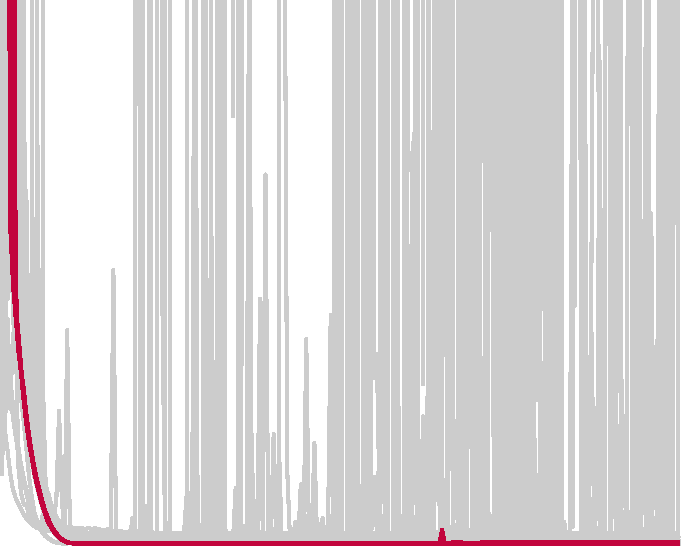
\includegraphics[width=0.4\textwidth]{figure4_a.pdf}};
	\end{tikzpicture}
	\begin{tikzpicture}
		\begin{axis}[
		table/col sep=comma,
		xlabel={(b) {cifar100}.},
		height=2.3in,
		width= 2.7in,
		ticklabel style={font=\small, fill=white},
		xticklabel style={rotate=90, anchor=near xticklabel},
		yticklabels={,,}
	    xtick={0,0.1,0.2,0.4,0.6,0.8,1},
    	xticklabels={dummy,0,50,100,150,200,250},
		]
		\end{axis}
		\node[inner sep=0pt] at (2.83,2.28) {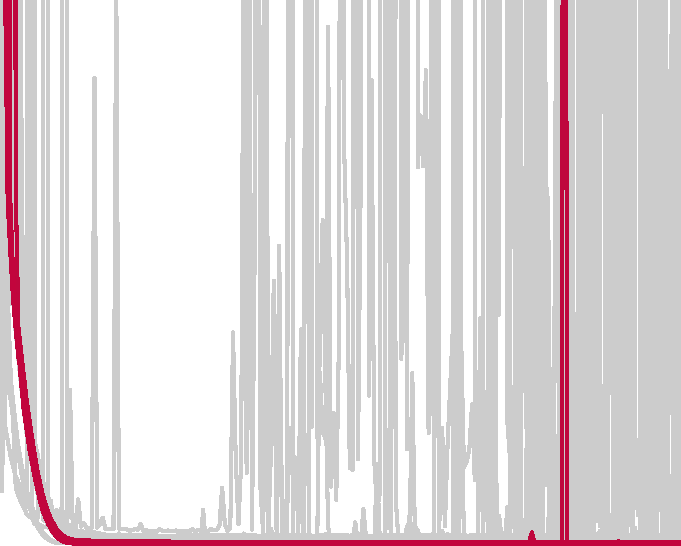
\includegraphics[width=0.4\textwidth]{figure4_b.pdf}};
	\end{tikzpicture}
\caption{The experiments show the mean squared error loss function on the validation dataset. We trained a total of $392$ neural nets ten times per dataset. Each line represents one neural net as an averaged loss function. The architecture can be found in Sect. \ref{subsec:invertibleneuralnets}, Appx. \ref{appx:invarch} and Fig. \ref{architecture}. The dimension of the net is chosen as a multiple of $2$, i.e. $2,4,6, \cdots, 784$. The {\color{brick} $\bullet$}--marked loss functions are parameterized above the determined threshold from Tab. \ref{stats}. The gray loss functions are below the defined threshold.}
\label{costfunctions}
\end{figure}

\section{Conclusions}
\label{sec:conclusion}
Based on the theory of Lie groups and persistent homology a method for invertible resnets was developed to parameterize them with good precision due to the assumption that the data lies on or near by some commutative Lie group. This forms an approximate solution for a special case of learning problems, allowing to restrict the domain to a commutative group. The initial problem could be simplified by decomposing the Lie group into a product space $\mathbb{R}^p \times \mathbb{T}^q$. The homology groups of the $q$-torus and the Euclidean space are well known. The application of fully invertible neural nets to resnets demonstrates our results on a different Lie group from Euclidean space. By applying Künneth's theorem the homology groups of the topological factor spaces could be connected with the ones of their product space. Using mean confident persistence landscapes the homology groups were estimated. A treshold was computed, see sect. \ref{sec:numericalexperiments}, which is determined by the state space dimension of the resets according to a representation up to homology equivalence. The mean persistence landscapes are particularly useful for short-lived isolated collections of data points, which in particular generate elements from homology classes at the beginning of the filtering and become visible at the lower left corner of the persistence landscapes, see Fig. \ref{homgroups} (a). The theoretical work was tested with numerical experiments on toy data. We do not limit the processing of the neural net within the layers to an abelian group. Instead, we assume that the net learns this structure from the input domain. This seems to hold, according to our experiments. Still, it can cause inaccuracies in the estimation of the dimensional treshold. The abelianization of the invertible layers would solve this problem.

\paragraph{Acknowledgements} The work is partially supported by Siemens Power and Gas. The authors would like to thank Noah Becker and David Haller for proofreading.

\paragraph{Code} The code can be found at: \href{https://github.com/karhunenloeve/Irhe}{https://github.com/karhunenloeve/Irhe}.
%
%
%
%
% ---- Bibliography ----
%
% BibTeX users should specify bibliography style 'splncs04'.
% References will then be sorted and formatted in the correct style.
%
\bibliographystylemain{splncs04}
\bibliographymain{biblio}
%
\newpage
\appendix
\section{Supplementary Material for Sect. \ref{sec:manifoldassumption}}
\label{a:mannilliegroup}
\subsection{Groups}
\label{a:groups}
\begin{definition}
A set $G$ together with a map $\mu: G \times G \rightarrow G$, $(x,y) \mapsto xy$ and an element $e = e_G$ is called group if the following conditions are fulfilled:
\begin{enumerate}
	\item[(1)] $(xy)z = x(yz)$ for all $x,y,z \in G$, thus the elements are associative,
	\item[(2)] $xe = ex = x$ for all $x \in G$, so there is a neutral element and
	\item[(3)] $\forall x \in G \; \exists \; x^{-1} \in G$, such that $xx^{-1} = x^{-1}x = e$. 
\end{enumerate}
\end{definition}

\begin{definition}{\cite[p.~196]{hilton2012course}}
Let $G$ be a group and contain a subset $H \subseteq G$. $G$ is called free group with basis $B$, if for each $H$ and each function $\psi: B \rightarrow H$ a unique homomorphism $\varphi: G \rightarrow H$ with $\varphi(x) = \psi(x)$ exists for all $x \in B$.
\end{definition}

\begin{example}
The most prominent example for a free group are the integers with addition $(\mathbb{Z},+)$ and basis $B = \{1\}$. Consider $\psi: B \rightarrow G$ with $g = \psi(1)$ and $g \in G$ and $\varphi(x) = g^n$ for each $n \in \mathbb{Z}$. Then $\varphi$ is the only group homomorphism of $(\mathbb{Z},+)$ into $G$, such that $\varphi(1)=\psi(1)$.
\end{example}

\begin{definition}
Let $\textbf{X} = \{X,\varphi_i\}_{i \in I}$ and $\textbf{Y} = \{Y,\psi_i\}_{i \in I}$ be two algebraic structures of the same type $\sigma = \{n_i\}_{i\in I}$, such that for each $i \in I$ and $n_i \in \mathbb{N}$, the arity of the fundamental operations is denoted with $\varphi_i$ and $\psi_i$. The projection $\varphi: \textbf{X} \rightarrow \textbf{Y}$ is called homomorphism, if for all $x_{i} \in X$
\begin{equation}
\varphi\left(f_i\left(x_{1},\cdots,x_{n}\right)\right) = g_i\left(\varphi\left(x_{1}\right),\cdots,\varphi\left(x_{n}\right)\right).
\end{equation}
\end{definition}

\begin{example}
The function $\varphi: \mathbb{Z} \rightarrow \mathbb{Z}/2\mathbb{Z}$ is a homomorphism of groups. The group $(\mathbb{Z}/2\mathbb{Z},+)$ is the quotient space that assembles all even integers to zero and all odd integers to one, where the respective equivalence class is defined.
\end{example}

\begin{remark}
Recalling group homomomorphisms and isomorphisms helps to gain proper intuition on chain and boundary groups. Isomorphisms from one algebraic structure to another exist if these two structures are considered to be essentially `equal'. A homomorphism is weaker. It preserves `some' of the structure. Since isomorphisms are homomorphisms, this preserved structure can be regarded as a kind of `subset'. Homomorphisms preserve operations, but allow elements of one algebraic structure to collapse into some elements of the other. 
\end{remark}

\begin{definition}
A subgroup $H \subseteq G$ is a group if a homomorphism $\varphi: G \rightarrow H$ exists, which maps $\varphi(e_G)$ to $e_H$ and $\varphi(xy)$ to $\varphi(x)\varphi(y)$ for all $x,y \in G$. A subgroup is called \emph{normal} if $xHx^{-1} = H$, for all $x \in G$.
\end{definition}

\begin{example}{\cite[p.~5]{van2003lie}}
Consider $\varphi:G\rightarrow H$ as a surjective group homomomorphism. Then $K := \ker \varphi$ is a normal subgroup of $G$. There is a unique map $\overline{\varphi}: G/K \rightarrow H$, which yields $\overline{\varphi} \circ \pi = \varphi$, with the canonical projection $\pi$. The \emph{factor map} $\overline{\varphi}$ is an isomorphism of groups.
\end{example}

\begin{proof}
Let $x \in G$ and $k \in K$. Then $\varphi(xkx^{-1})$ $=$ $\varphi(x)\varphi(k)\varphi(x^{-1})$ $=$ $\varphi(x)e_H\varphi(x)^{-1}$ $=$ $e_H$, thus $xkx^{-1}$ is an element of $\ker \varphi = K$. It follows that $xKx^{-1} \subset K$. Due to the properties of the neutral element $x^{-1}Kx \subset K$, i.e. $K \subset xKx^{-1}$, we get $K = xKx^{-1}$. \qed
\end{proof}

\begin{remark}
Similar as subsets behave to sets, \emph{subgroups} behave to groups. 
\end{remark}


\subsection{Lie groups}
\begin{definition}
Let $G$ be a commutative abelian Lie group. The exponential map $\exp := \exp_G : T_eG \rightarrow G$ maps from the tangent space $T_eG$ in $e$ into the group $G$. It also maps in every point into $G$ due to homogeneity. It is defined as $\exp(\mathfrak{X}) = \alpha_{\mathfrak{X}} (1)$ for a left invariant vector field $\mathfrak{X} \in T_eG$ and a maximal integral curve $\alpha_{\mathfrak{X}}$ with a starting point $e$. For all $s,t \in \mathbb{R}$ and each $\mathfrak{X} \in T_eG$ the exponential map fulfils the properties
\begin{itemize}
	\item[(a)] $\exp(s\mathfrak{X}) = \alpha_{\mathfrak{X}}(s)$,
	\item[(b)] $\exp(s+t) \mathfrak{X} = \exp(s\mathfrak{X}) \exp(t \mathfrak{X})$.
\end{itemize}
\end{definition}

\begin{proof}
Let $\gamma(t) = \alpha_{\mathfrak{X}}(st)$ be a curve. Then $\gamma(0) = e$ and
\begin{align}
	\frac{d}{dt}\gamma(t) = s\dot{\alpha}_{\mathfrak{X}}(st) = s v_{\mathfrak{X}}(\alpha_{\mathfrak{X}}(st)) = v_{s\mathfrak{X}}(\gamma(t)).
\end{align}
Let $\mathfrak{X} \in T_eG$, then the integral curve $\alpha_{\mathfrak{X}}$ is defined on $\mathbb{R}$. Let $y \in G$ and $\alpha_1(t) = y\alpha(t)$. Differentiating with respect to $t$ yields
\begin{align}
	\frac{d}{dt}\alpha_{1}(t) = T_{\alpha(t)}y \frac{d}{dt} \alpha(t) = T_{\alpha(t)} y v_{\mathfrak{X}}(\alpha(t)) = v_{\mathfrak{X}}(\alpha_1(t))
\end{align}
by the left invariance of $v_{\mathfrak{X}}$. So $\alpha_1$ is also an integral curve for $v_{\mathfrak{X}}$. Let $I$ be the domain of $\alpha_{\mathfrak{X}}$ and $t_1 \in I$ with $x_1 = \alpha_{\mathfrak{X}}(t_1)$. Then $\alpha_1(t) := x_1 \alpha_{\mathfrak{X}}(t)$ is an integral curve for $v_{\mathfrak{X}}$ with starting point $x_1$ given by $\alpha_2: t \mapsto \alpha_{\mathfrak{X}}(t+t_1)$. The integral curve has domain $I-t_1$. We conclude that $I \subset I-t_1$. It follows that $s+t_1 \in I$ for all $s, t_1 \in I$ so $I$ must be equal to $\mathbb{R}$.

For a fixed $x \in \mathbb{R}$ we get $\gamma: t \mapsto \alpha_{\mathfrak{X}}(s)\alpha_{\mathfrak{X}}(t)$ as maximal integral curve for $v_{\mathfrak{X}}$ with starting point $\alpha_{\mathfrak{X}}(s)$. On the other hand, the same applies to $\epsilon: t \mapsto \alpha_{\mathfrak{X}}(s+t)$. Thus $\gamma = \epsilon$ and we get
\begin{align}
	\exp((s+t)\mathfrak{X}) = \alpha_{\mathfrak{X}}(s+t) = \alpha_{\mathfrak{X}}(s) \alpha_{\mathfrak{X}}(t) = \exp(s\mathfrak{X}) \exp(t\mathfrak{X}).
\end{align} \qed
\end{proof}

\begin{remarkdef}
The exponential map is a smooth map $\exp_G: T_eG \rightarrow G$ and a local diffeomorphism around $0$.
\end{remarkdef}

A Lie group $G$ is also a smooth manifold, as defined in Sect. \ref{liegroups}. Its tangential space is a linear space, which we denote as $\mathfrak{g}$.

\begin{definition}
Each linear space $\mathfrak{g}$ equipped with a bilinear form $[\cdot,\cdot]: \mathfrak{g} \times \mathfrak{g} \rightarrow \mathfrak{g}$ is called Lie algebra, if the bilinear form, also called Lie bracket, is 
\begin{itemize}
	\item[(1)] antisymmetric, i.e. $[\mathfrak{X}, \mathfrak{Y}] = -[\mathfrak{Y}, \mathfrak{X}]$ and the
	\item[(2)] Jacobi identity holds $[\mathfrak{X},[\mathfrak{Y},\mathfrak{Z}]] = [\mathfrak{Y},[\mathfrak{Z},\mathfrak{X}]] + [\mathfrak{Z},[\mathfrak{X},\mathfrak{Y}]]$, for all $\mathfrak{X}, \mathfrak{Y}, \mathfrak{Z} \in \mathfrak{g}$.
\end{itemize}
\end{definition}

\begin{remarkdef}
For a Lie group $G$ with subgroup $H$ both properties are equivalent \cite[pp.~25-27]{van2003lie}.
\end{remarkdef}

\begin{propositionsec}{\cite[p.17]{van2003lie}} Let $G$ be a Lie group and $H$ a subgroup. Then the following properties are equivalent:
\begin{enumerate}
	\item[(1)] There is an open neighborhood $U$ of $e$ such that $U \cap H = \{e\}$.
	\item[(2)] The group $H$ is discrete.
	\item[(3)] For each compact subset $C \subset G$ the intersection $C \cap H$ is finite.
	\item[(4)] The group $H$ is a closed Lie subgroup with Lie algebra $\{0\}$.
\end{enumerate}
\end{propositionsec}
\begin{proof}Take any element $h \in H$. Then $hU$ is an open neighbourhood of $h$ in $G$. $hU \cap H = h(U\cap h^{-1}H)$ and from the group structure of $H$ it follows that $h(U\cap h^{-1}H) = h(U \cap H) = \{h\}$.

Choose $U$ as an open neighborhood centered around $e = e_G$, such that $U \cap H = \{e\}$. Let $g \in G$ be a point in the closure $\overline{H}$. Then there is a sequence $\{h_i\}$ in $H$ which converges to $g$. It follows that $h_{i+1}h_i^{-1} \rightarrow gg^{-1} = e$, with $i \rightarrow \infty$. For an $i$ large enough, $h_{i+1}h_i^{-1} \in U \cap H = \{e\}$, i.e. $h_i = h_{i+1}$. The sequence $h_i$ becomes stationary after a certain index. Therefore $h_i = g$ for some $i$. We conclude that $g \in H$ for any $g$. Further we see that $\overline{H} \subset H$ and therefore $H$ is closed. Since $H$ is closed, the intersection $H \cap C$ is also closed, thus compact. For a $c \in H \cap C$ we choose an open neighborhood $cU$ in $G$, such that $cU \cap H = \{c\}$. Then $\{cU \; | \; c \in H \cap C\}$ is an open cover of $H \cap C$ with no proper subcover. Since $H \cap C$ is compact, the cover must be finite and thus $H \cap C$ is finite.

Let $g \in G$ a point in the closure $\overline{H}$. We choose a compact neighborhood $C$ around $g$, such that $g$ lies in the closure $\overline{H \cap C}$. The latter is finite, thus closed. Therefore $g$ is in the closure $\overline{H \cap C} \subset H$ and contained in $H$. We conclude that $H$ is a closed Lie subgroup. Let $\mathfrak{g}$ be the Lie algebra of $H$ consisting of $\mathfrak{X} \in \mathfrak{g}$ with $\text{exp}(\mathbb{R}\mathfrak{X}) \subset H$. A local diffeomorphism $\text{exp}: \mathfrak{g} \rightarrow G$ to $0$ gives an open neighborhood $\mathfrak{o}$ around $0$ in $\mathfrak{g}$. The exponential function is injective on $\mathfrak{o}$. If we take $\mathfrak{X} \in \mathfrak{g} \setminus \{0\}$, then there is an $\epsilon > 0$, such that $[-\epsilon, \epsilon]\mathfrak{X} \subset \mathfrak{o}$. We define a curve $\gamma: [\epsilon,\epsilon] \rightarrow G$, $t \mapsto \text{exp}(t\mathfrak{X})$, with compact image. Thus $\Ima(\gamma) \cap H$ and $\{t \in [-\epsilon,\epsilon] \; | \; \text{exp}(t \mathfrak{X}) \in H\}$ are finite. Hence, $\mathfrak{X} \notin \mathfrak{h}$ and $\mathfrak{h} = \{0\}$. 

$H$ is a closed smooth submanifold of $\mathfrak{X}$, where $\dim H = 0$. It follows that an open neighborhood $U$ exists from $e$ to $G$, such that $U \cap H = \{e\}$. \qed
\end{proof}

\subsection{Decomposition of Connected Commutative Lie groups}
\label{decomposition}
\begin{theorem}{\cite[p.~116,~p.~26]{onishchik1993lie,van2003lie}}
\label{connectedcommutativeliegroupdecomposition}
Every connected commutative (or in other words abelian) Lie group $G$ is isomorphic to some product space $\mathbb{R}^p \times \mathbb{T}^q$ with $\dim G = p+q$, i.e. $G \simeq \mathbb{R}^p \times \mathbb{T}^q$.
\end{theorem}

\begin{proof}
Choosing $G$ as a connected abelian Lie group, the Lie algebra $\mathfrak{g}$ is commutative, such that $[\mathfrak{X}, \mathfrak{Y}] = 0$ for all $\mathfrak{X}, \mathfrak{Y} \in \mathfrak{g}$. It follows that the exponential map $\text{exp}(\mathfrak{X})\text{exp}(\mathfrak{Y}) = \text{exp}(\mathfrak{X}+\mathfrak{Y})$ is given for all $\mathfrak{X}, \mathfrak{Y} \in \mathfrak{g}$. Thus $\text{exp}: \mathfrak{g} \rightarrow G$ is a Lie group homomorphism from $(\mathfrak{g},0,+)$ to $G$. It follows that $\text{exp}(\mathfrak{g})$ is a subgroup of $G$, thus $\text{exp}(\mathfrak{g}) = G_e$. Since $G$ is connected, $G = G_e$. Therefore $\Ima \text{exp}(\mathfrak{g}) = G$ and $\text{exp}: \mathfrak{g} \rightarrow G$ is a surjective Lie group homomorphism. If $\Omega$ is the closed subgroup $\text{ker}(\text{exp})$ of $\mathfrak{g}$, then according to the Isomorphism Theorem for groups: $G \simeq \mathfrak{g}/\Omega$ \cite[pp.~5-7]{van2003lie}. Since $\text{exp}$ is a local diffeomorphism at $0$, there is an open neighborhood $\Gamma$ of $0$ in $\mathfrak{g}$ for which $\text{exp}$ is an injective map. It follows that $\Gamma \cap \Omega = \{0\}$. Thus $\Omega$ is a discrete subgroup of $\mathfrak{g}$. 

We need a corresponding basis for a discrete group consisting of finite-dimensional linear independent elements with coefficients in $\mathbb{Z}$.

\begin{lemma}{\cite[p. 27]{van2003lie}}
A subset of a finite dimensional linear space $V$ can be written by linear independent components $\omega_1, \cdots, \omega_p$ of $V$ as a direct sum with coefficients in $\mathbb{Z}$, such that $\Omega = \mathbb{Z}\omega_1 \oplus \cdots \oplus \mathbb{Z}\omega_p$.
\end{lemma}

\begin{proof}
We show that by induction and start with $\dim V = 1$. Choosing a basis, we identify $V$ with $\mathbb{R}$. Then $\Omega$ is a discrete subgroup of $\mathbb{R}$. We assume that $\Omega \neq \{0\}$, then there is an element $x \in \Omega \setminus \{0\}$ with $x > 0$. The section $\Omega \cap [0,x]$ is finite and therefore contains a smallest element $\omega$. The section $\Omega \; \cap \; ]0,1[\omega$ is equal to the empty set, thus $\mathbb{Z} \omega \subset \Omega$. Next we consider an element $y \in \Omega$, then $y \not\in \mathbb{Z}\omega$ would mean that $y \; \in \; ]n,n+1[\omega$ for a corresponding $n \in \mathbb{Z}$. This means that $y-nx \in \Omega \; \cap \; ]0,1[ \omega = \emptyset$. This in turn implies $\Omega \subset \mathbb{Z}\omega$. Thus $\Omega = \mathbb{Z}\omega$.

For the general case we use the idea from van den Ban's proof \cite[p.27]{van2003lie}. We assume that $\dim V = n$ for any $n > 1$. In the trivial case $p = 0$ and $\Omega = \{0\}$ holds. For $\omega \in \Omega \setminus \{0\}$ the intersection $\mathbb{R} \omega \cap \Omega$ is discrete in $\mathbb{R} \omega$, i.e. an integer multiple $\mathbb{Z}\omega_1$. We choose a linear subspace $U \subset V$, in order that $\mathbb{R}\omega_1 \oplus U = V$, with the canonical projection $\pi: U \rightarrow V$ and $C \subset U$ as compact subset:
\begin{align}
\pi^{-1}\left(C\right) &= \mathbb{R} \omega_1 + C = \left([0,1] \omega_1 + C\right) + \mathbb{Z}\omega_1,\\
\implies \pi\left(\Omega\right) \cap C &= \pi\left(\left(C + [0,1] \omega_1\right) \cap \Omega + \mathbb{Z}\omega_1\right)\\
&= \pi\left(\left(C + [0,1]\omega_1\right) \cap \Omega\right). 
\end{align}
The set $C$ is compact, so is $C + [0,1] \omega_1$. It follows that the intersection $(C + [0,1] \omega_1) \cap \Omega$ is also compact. Thus $C$ is a discrete compact subset of $U$. By induction there are linearly independent elements $\overline{\omega}_2, \cdots, \overline{\omega}_p$ of $\pi(\Omega)$, such that $\pi(\Omega) = \mathbb{Z} \overline{\omega}_2 \oplus \cdots \oplus \mathbb{Z}\overline{\omega}_p$. We choose $\pi(\omega_i) = \overline{\omega}_i$, then the elements $\omega_1, \cdots, \omega_p$ are linearly independent and we get the basis $\Omega = \mathbb{Z}\omega_1 \oplus \cdots \oplus \mathbb{Z}\omega_p$. \qed
\end{proof}

Since $\mathfrak{g}$ is a linear space, we can extend the basis $\mathbb{Z}\omega_1 \oplus \cdots \oplus \mathbb{Z} \omega_n$ to the whole Lie algebra $\mathfrak{g}$. Thus we get a linear isomorphism $\varphi: \mathfrak{g} \rightarrow \mathbb{R}^n$, where $\mathbb{R}^n \simeq \mathbb{R}^p \times \mathbb{R}^q$ with $p+q = n$. The map $\text{exp} \circ \varphi^{-1}: \mathbb{R}^n \rightarrow G$ is a surjective Lie group homomorphism, i.e. a group homomorphism that is smooth, with smooth inverse. According to the Isomorphism Theorem for groups, this group also factorizes by a bijective group homomorphism \cite[pp.~5-7]{van2003lie}:
\[
\begin{tikzcd}[column sep=huge]
    \displaystyle \mathfrak{g}
    \arrow[swap]{r}{\varphi}
    \arrow[bend left=25]{rr}{\text{exp}}
    \arrow[swap]{dr}{\pi \; \circ \; \varphi}
&   \mathbb{R}^p \times \mathbb{R}^q
    \arrow{d}{\pi}
    \arrow[swap]{r}{\text{exp} \; \circ \; \varphi^{-1}}
&   G\\	
&   (\mathbb{R})^p \times \mathbb{R/\mathbb{Z}}^q 
	\arrow[swap]{ur}{\overline{\text{exp} \; \circ \; \varphi^{-1}}}
\end{tikzcd}
\]
The canonical map $\pi: \mathbb{R}^n \simeq \mathbb{R}^p \times \mathbb{R}^q \rightarrow \mathbb{R}^p \times (\mathbb{R}/\mathbb{Z})^q$ is locally diffeomorphic and $\overline{\text{exp} \circ \varphi^{-1}} \circ \pi$ as well. Due to the homogeneity of commutative lie groups, the map is everywhere a diffeomorphism. The projection $\overline{\text{exp} \; \circ \; \varphi^{-1}}$ is bijective, thus also a diffeomorphism and thus an isomorphism of Lie groups. By definition $\mathbb{R}^q/\mathbb{Z}^q \simeq (\mathbb{R}/\mathbb{Z})^q \simeq \mathbb{T}^q$ and the proof follows. \qed
\end{proof}

\section{Supplementary Material for Sect. \ref{sec:persistenthomology}}
\label{persistenthomologyproofs}
\subsection{Properties of Simplicial Complexes}
\begin{definition}
A simplicial complex $K$ is \textit{connected} if it cannot be composed of a disjoint union of two or more non-empty subcomplexes.
\end{definition}

\begin{definition}
An embedded simplicial complex is \emph{path-connected} if there is a path from any vertex to any other as a composition of $1$-simplices.
\end{definition}

\begin{propositionsec}
A simplicial complex $K$ is path-connected if it is connected and vice versa. Thus the notions are equivalent for simplicial complexes.
\end{propositionsec}

\begin{proof}
Assume $K$ is path-connected and not connected. Choose two subcomplexes $U,V \subset K$ with $U \cup V = K$. Choose a vertex $u_0 \in U$ and $v_0 \in V$. Thus a path from $u_0$ to $v_0$ exists, due to the path-connectedness of the simplicial complex. If $u_i$ is the last vertex in $U$, then the vertex $u_{i+1}$ can be contained neither in $U$ nor in $V$, due to the disjoint decomposition of the simplicial complex. This contradicts the assumption that it is path-connected. 

Consider two vertices $u,v \in K$ that are not path-connected. Define $U,V \subset K$ as path-connected subcomplexes containing $u\in U$ and $v \in V$.  Choose $w \in U \cap V \neq \emptyset$, then there is a path from $u$ to $w$ and also from $w$ to $v$. A composition of paths gives a path from $u$ to $v$, which contradicts the assumption that $u$ and $v$ are not path-connected. Thus $U \cap V = \emptyset$ and $K$ is not connected.\qed
\end{proof}

\subsection{Direct Sums of Homology Groups}
\label{directsums}
\begin{theorem}{\cite[p.~109]{hatcher2002algebraic}}
The $k$-th simplicial homology group $H^{\Delta}_n(K(X))$ of a simplicial complex $K$ for a field $\mathbb{F}$ is isomorphic to the direct sum of the homology groups of all subcomplexes on its filtration, i.e. $H^{\Delta}_n(K(X)) \simeq \bigoplus_{i \in I} H^{\Delta}_n(K^{\omega_{i}}(X))$.
\end{theorem}

\begin{proof}
Let $\{K^{\omega_{i}}\}_{i \in I}$ be the set of all connected components of the simplicial complex $K(X)$ of a point set $X$ and $H^{\Delta}_k\left(K\left(X\right)\right)$ its simplicial homology groups. We denote the homology groups of the components with $H_k^{\Delta}(K^{\omega_{i}}(X))$. With $C_k(K^{\omega_{i}}(X))$, we denote the group of $k$-chains for the connected components of the simplicial complex. Then $C_k(K^{\omega_{i}}(X)) \subseteq C_k(K(X))$ is a subgroup for all $i$.

\begin{lemma}
The group of $k$-chains can be written as a direct sum of the connected components, i.e. $C_k(K(X)) \simeq \bigoplus_{i \in I} C_k(K^{\omega_{i}}(X))$. This also applies to the lower chain groups.
\end{lemma}

\begin{proof}
Using the boundary operator, which is a homomorphism of groups, we get $C_{k-1}(K(X)) \simeq \bigoplus_{i \in I} \partial_k(C_{k}(K^{\omega_{i}}(X)))$. An element in the $(k+1)$-th chain group $v \in C_{k+1}(K(X))$ is represented by $v = \sum_{i \in I} v_{\omega_{i}}$. Thus $\partial_{k+1}(v) \in C_{k}(K(X))$ can be broken down to $\partial_{k+1}(v) = \sum_{i \in I} \partial_{k+1}(v_{\omega_{i}})$ where $v_{\omega_{i}} \in C^\omega_{k+1}(K^{\omega_{i}}(X))$.\qed
\end{proof}

The groups of boundaries can also be decomposed. The kernel of $C_k(K^{\omega_{i}}(X))$ can be written as $\ker \partial_k(C_k(K^{\omega_{i}}(X)))$ $= \ker \partial_k(C_k(K(X)))$ $\cap$ $C_k(K^{\omega_{i}}(X))$.
\begin{align}
	\ker \partial_k &\simeq \bigoplus_{i \in I} \partial_k\left(C_k\left(K^{\omega_{i}}(X)\right)\right), \text{which implies}\\
	&\Rightarrow \frac{\ker \partial_k\left(C_k\left(K\left(X\right)\right)\right)}{\Ima \partial_{k+1}\left(C_{k+1}\left(K\left(X\right)\right)\right)} \simeq \bigoplus_{i \in I} \frac{\ker \partial_k(C_k(K^{\omega_{i}}(X)))}{\Ima \partial_{k+1}(C_{k+1}(K^{\omega_{i}}(X)))}\\
	&\Rightarrow H^{\Delta}_k(K(X)) \simeq \bigoplus_{i \in I} H^{\Delta}_k(K^{\omega_{i}}(X)).
\end{align}
\qed
\end{proof}

\begin{remarklem}
We obtain an isomorphism for the singular homology groups from the homology groups of the set of path components. This can be thought of as a direct sum of all `loops' from every possible path component in space.
\end{remarklem}

\begin{definition}
A \emph{path component} of a topological space $X$ is an equivalence class under the equivalence relation $x \sim y$ if there is a path from $x$ to $y$.
\end{definition}

\begin{remarkdef}
Since for simplicial complexes the property to be connected corresponds to path-connectedness, the coordinatewise sum of the connected components is a generator of the whole group.
\end{remarkdef}

\begin{theorem}{\cite[p.~129]{hatcher2002algebraic}}
Let $X$ be a topological space and $\{X^{\omega_{i}}\}_{i \in I}$ a set of path components of $X$ and $\imath_{\omega_{i}}: X^{\omega_{i}} \hookrightarrow X$ the inclusion. Then the maps $(\imath_{\omega_{i}})_\star: H_k(X^{\omega_{i}}) \hookrightarrow H_k(X)$ for each $k \geq 0$ induce an isomorphism between the direct sum of the homology groups of all simplicial subcomplexes and the homology groups of $X$:
\begin{equation}
	\bigoplus_{i \in I} H_k(X^{\omega_{i}}) \rightarrow H_k(X).
\end{equation}
\end{theorem}

\begin{proof}Consider $C_k(X^{\omega_{i}})$ to be the free abelian group with basis $\{\sigma: \Delta^k \rightarrow X^{\omega_{i}}\}$ of all singular simplices in $X^{\omega_{i}}$. A generator $\sigma \in C_{k}(X^{\omega_{i}})$ is a simplex in $X$ composed with the inclusion $\imath_{\omega_{i}}$, i.e. $(\imath_{\omega_{i}})_\star: C_k(X^{\omega_{i}}) \rightarrow C_k(X)$, $\sigma \mapsto \imath_{\omega_{i}} \circ \sigma$. If we take all $i \in I$, we can exhaust $C_k(X)$, which results in the isomorphism $\psi: \bigoplus_{i \in I} H_k(X^{\omega_{i}}) \rightarrow H_k(X)$ at chain level. Taking an element $x \in \bigoplus_{i \in I} C_k(X^{\omega_{i}})$ we get a finite sum of the functions $\sigma_1, \cdots, \sigma_n$ with their coefficients $z_1, \cdots, z_n \in \mathbb{Z}$, i.e. $x = \sum_{i=1}^{n} z_i\sigma_i$ and apply the group homomomorphism $\psi$, resulting in $\psi(x) = \sum_{i=1}^{n} z_i \imath_{\omega_i}(\sigma_i)$. Given a generator $\sigma: \Delta^k \rightarrow X$, we know that $\Delta^k$ is connected and $\sigma$ is a continuous function. Thus $\sigma(\Delta^k)$ is contained in a connected component of $X$, namely $\sigma \in C_k(X^{\omega_{j}})$ and $\sigma = \psi(\sigma)$, thus $\psi$ is surjective.\qed
\end{proof}

\subsection{Equivalence of Simplicial and Singular Homology}
\label{simplicialsingularequivalence}
\begin{theorem}{\cite[p.~128]{hatcher2002algebraic}}
Let $k \in \mathbb{Z}$ and $H^\Delta_k(K(X))$ the simplicial $k$-th homology group over a triangulable topological space $X$ and $K$ the triangulation. Let $H_k(X)$ be the respective singular homology group. Then the map $H^{\Delta}_k(K(X)) \rightarrow H_k(X)$ is an isomorphism of groups.
\end{theorem}

\begin{proof}
We follow the proofs of \cite[p.~128, pp.~190-192]{hatcher2002algebraic,munkres2018elements} and start from the perspective of the simplicial homology groups by choosing $K(X)$ as a simplicial complex and $K(X^n)$ as the $n$-skeleton of $X$, which consists of all simplices of dimension $n$ or less. Thus, with $K(X^{n-1}) \subset K(X)$ we obtain the following commutative diagram of exact sequences, for which $\ker(\psi_i) = \Ima(\psi_{i+1})$:
\[
\begin{tikzcd}
& {H^{\Delta}_{k+1}((K(X^n),K(X^{n-1})))} \arrow[d, "\sigma_i"] \arrow[r, "\psi_i"]
& H^{\Delta}_{k}(K(X^{n-1})) \arrow[d, "\sigma_j"] \arrow[dd, bend left=80, "\psi_j"] \\
& {H_{k+1}((X^n,X^{n-1}))} \arrow[r, "\psi'_i"]
& H_{k}(X^{n-1}) \arrow[dd, bend left=80, "\psi'_j"]\\
H^{\Delta}_{n-1}(K(X^{n-1})) \arrow[d, "\sigma_m"]
& {H^{\Delta}_{k}((K(X^n),K(X^{n-1})))} \arrow[l,"\psi_k"] \arrow[d, "\sigma_l"]
& H^{\Delta}_{k}(K(X^n)) \arrow[l, "\psi_l"] \arrow[d, "\sigma_k"]\\
H_{k-1}(X^{n-1})
& {H_{k}((X^n,X^{n-1}))} \arrow[l,"\psi'_k"]
& H_{k}(X^{n}) \arrow[l,"\psi'_l"]
\end{tikzcd}
\]
The quotient space $X^n/X^{n-1}$ contains only simplices of dimension $n$. For $k \neq n$ the group $C_k((X^n,X^{n+1}))$ is zero. For $k = n$, the group $C_k((X^n,X^{n+1}))$ is free and commutative with a basis consisting of $k$-simplices. The cycles $\ker \partial_k$ are a subgroup of $C_k((X^n,X^{n+1}))$ and the boundary group $\Ima \partial_{k+1}$ is empty. We conclude that $H^{\Delta}_k((K(X^n),K(X^{n-1})))$ has a description like $C_k((X^n,X^{n-1}))$.

The continuous maps $\sigma: \Delta^n \rightarrow X$ into the topological space $X$ give the map $\psi: \coprod_i(\Delta^n_i,\Delta^{n-1}_i) \rightarrow (X^n,X^{n-1})$ and for the simplicial quotient spaces $\psi_{\star}: \coprod_i \Delta^n_i / \coprod_i \Delta^{n-1}_i \rightarrow X^n/X^{n-1}$. In view of these homeomorphisms, the following isomorphism of homology groups results:
\begin{align}
	H_k(\coprod_i \Delta^n_i / \coprod_i \Delta^{n-1}_i) \simeq H_k(X^n / X^{n-1}).
\end{align}

A consequence of the Excision Theorem is the existence of an isomorphism $H_k((X,V)) \rightarrow H_k(X/V)$ for all good pairs $(X,V)$ \cite[pp.~175-182]{munkres2018elements}.

\begin{theorem}
Given the topological spaces $U \subset V \subset X$ for which the closure $\overline{U} \subset \interior{V}$ is in the interior of $V$, the embedding $(X-U,V-U) \hookrightarrow (X,V)$ induces an isomorphism $H_k((X-U, V-U)) \rightarrow H_k((X,V))$ for all $k \in \mathbb{Z}$.
\end{theorem}

\begin{proof}
For a proof we refer to \cite[pp.~175-182]{munkres2018elements}. \qed
\end{proof}

\begin{remarktheo}
Recall that the notation $(X^{n},X^{n-1})$ denotes a topological pair, i.e. a shorthand to indicate an inclusion $\imath: X^{n-1} \hookrightarrow X^n$. 
\end{remarktheo}
\begin{remarktheo}
As a reminder, a good pair $(X,V)$ is given if there is an open neighborhood $W \subset X$ with $V \subset W$ such that this deformation retracts onto $V$. 
\end{remarktheo}

Applying transitivity of group operations yields
\begin{align}
	H_k\left(\coprod_i\left(\Delta^n_i,\Delta^{n-1}_i\right)\right) &\simeq H_k\left(\coprod_i \Delta^n_i/\coprod_i \Delta^{n-1}_i\right),\\
	H_k\left(\coprod_i \Delta^n_i/\coprod_i \Delta^{n-1}_i\right) &\simeq H_k\left(\left(X^n,X^{n-1}\right)\right),\\
	H_k\left(\left(X^n,X^{n-1}\right)\right) &\simeq H_k(X^n / X^{n-1}).
\end{align}
We see, that $H_k((X^n,X^{n-1}))$ is zero, for $k \neq n$ and a free abelian group, on the basis of the cycles given by the continuous map $\sigma: \Delta^n \rightarrow X$. It follows that the map $H^\Delta_k((K(X^n),K(X^{n-1}))) \rightarrow H_k((X^n,X^{n-1}))$ is an isomorphism.

In the commutative diagram of simplicial and singular homology groups above, the maps $\sigma_i$ and $\sigma_m$ are isomorphisms. By induction $\sigma_j$ and $\sigma_l$ are also isomorphisms. It remains to be shown that $\sigma_k$ is also an isomorphism. For this purpose we use the Five Lemma \cite{pryde1977five}, from which follows that $\sigma_k$ is an isomorphism and therefore the map $H^{\Delta}_k(K(X^n)) \rightarrow H_k(X^n)$ is an isomorphism. \qed
\end{proof}

\subsection{Singular Homology and Smooth Manifolds}
To complete the argument we use ideas from a proof of de Rham`s Theorem. De Rham's Theorem manifests the fundamental connection of the analytic and topological properties of a smooth manifold, where the pairing of differential forms and singular chains gives an isomorphism from $k$-th de Rham cohomology to $k$-th singular homology and an isomorphism into simplicial homology.

\begin{theorem} The de Rham cohomology of a smooth, oriented and trianguliable manifold $H_{k}^{\text{dR}^{*}}(M)$ has an isomorphism to the real homology group $H_k(K(M);\mathbb{R})$, e.g. calculated by a singular \v{C}ech complex $K$ on some smooth manifold $M$ with real coefficients.
\end{theorem}

\begin{proof}
For a complete proof we refer to  \cite[Chap.~18, Sect.~V.9]{lee2013smooth,bredon2013topology}.
\end{proof}

\begin{theorem}
\label{singularsmoothhomgroup}
The $k$-th smooth singular homology group is defined as
\begin{equation}
	H_{k}^{\infty} (M) = \frac{\ker\left(\partial: C_{k}^{\infty} \rightarrow C_{k-1}^{\infty}\left(M\right)\right)}{\Ima\left(\partial: C_{k+1}^{\infty}\left(M\right) \rightarrow C_{k}^{\infty}\left(M\right)\right)},
\end{equation}
and gives an isomorphism into the singular homology groups on $M$, such that the map $\imath_{\star}: H_{k}^{\infty}(M) \rightarrow H_k(M)$ is an isomorphism of groups.
\end{theorem}

\begin{remarktheo}
For the free abelian group of $k$-chains $C_k(M)$ created by smooth $k$-simplices on $M$ we introduce the notation $C_k^{\infty}(M)$. These are formal sums of finitely many smooth $k$-simplices. The boundary of a smooth $(k+1)$-simplex is thus a smooth $k$-chain.
\end{remarktheo}

\begin{proof}
Let $U \subset \mathbb{R}^n$ be a subset of the Euclidean space and $f: U \rightarrow M$ a smooth map into the manifold $M$. The map is said to be smooth in $p \in U$ if there is a smooth extension of $f$ to an open neighborhood of $p$. If $p$ is arbitrary, then $f$ is smooth in $M$. The standard basis vectors $\Delta_i$ form a smooth $k$-simplex $\Delta^k := [v_0, \ldots, v_k] \subset \mathbb{R}^n$, with a smooth map $\sigma: \Delta^k  \rightarrow M$.

The inclusion $\imath: C_{k}^{\infty}(M) \hookrightarrow C_k(M)$ satisfies $\imath \circ \partial = \partial \circ \imath$, from which we can see, that it induces a map $\imath_{\star}: H_{k}^{\infty}(M) \rightarrow H_k(M)$, for which $\imath_{\star}[x] = [\imath(x)]$.

\begin{lemma}
For the simplex $\Delta^k \subset \mathbb{R}^n$ with the standard basis vectors as vertices, let $\sigma: \partial \Delta^k \rightarrow M$ be the continuous map with a restriction to the boundary of each face. Then $\sigma$ is smooth as a function from $\partial \Delta^k$ into $M$.
\end{lemma}

\begin{proof}
We follow the proof of \cite[Lem.~2.1]{parkproof}. Let $0 \leq i \leq k$ and $\hat{v}_i$ denote the boundary face opposite of $\partial_{i} \Delta^k = [v_0, \cdots, \hat{v}_i, \cdots, v_k]$, where the primer represents the omitted element by the boundary operator. For each $i$ and each $v \in\partial_{i} \Delta^k$ we seek an open neighborhood $v \in U_v \subseteq \mathbb{R}^n$ and a smooth extension $\tilde{\sigma}: U_v \rightarrow M$ of $\sigma$ such that $\tilde{\sigma}$ restricted to $U_v \cap \partial_{i}\Delta^k$ corresponds exactly to $\sigma$.

\begin{proposition}
For each $v \in \partial \Delta^k$ a smooth extension $\tilde{\sigma}$ into $M$ exists.
\label{smoothextension}
\end{proposition}

\begin{proof}
We follow the proof of \cite[Lem.~2.1]{parkproof}. The element $v$ is contained in at least one boundary face of $\Delta^k$, but cannot be contained in all of them. This means that the boundary faces $\partial_1 \Delta^k, \cdots, \partial_j \Delta^k$ for $1 \leq j \leq k$ contain $v$. In particular $v$ is not contained in $\partial_0 \Delta^k$. Let $U = \bigcap_{i=1}^{j} U_i$ be the intersections for each possible $v \in \partial_i\Delta^k$. Using the induction hypothesis, we show that there is a smooth map $\tilde{\sigma}: U \rightarrow M$, whose restriction to $U \cap \left (\bigcup_{i=1}^j \partial_i \Delta^k \right)$ matches $\sigma$. This property is shown locally, such that for small enough $U$, $\sigma$ maps $U$ to a coordinate chart of $f(v)$, which in turn can be identified diffeomorphically as a subspace of $\mathbb{R}^n$. For $j=1$ the proof is trivial, thus assume that $j > 1$ and that a smooth map $\tilde{\sigma}_0 : U \rightarrow M$ exists, whose restriction to $U \cap \left( \bigcup_{i=1}^j \partial_i \Delta^k \right)$ matches $\sigma$. We define $\tilde{\sigma}: U \rightarrow M$ with
\begin{align}
	&\tilde{\sigma} \circ \left(v_1,\cdots,v_{i-1},0,v_{i+1},\cdots,v_n\right) = \\
	= \; &\tilde{\sigma}_0 \circ \left( v_1, \cdots, v_m\right) - \tilde{\sigma}_0 \circ  \left(v_1,\cdots,v_{j-1},0,v_{j+1},\cdots,v_m \right) + \\
	& + \tilde{\sigma}_j\circ \left(v_1,\cdots,v_{j-1},0,v_{j+1},\cdots,v_m \right).
\end{align}
For each $1 \leq i \leq j -1$ the restriction $\tilde{\sigma}$ to $U \cap \partial_i \Delta^k$ is given by
\begin{align}
&\tilde{\sigma} \circ \left(v_1,\cdots,v_{i-1},0,v_{i+1},\cdots, v_n\right) = \\
= \; &\tilde{\sigma}_0 \circ \left(v_1, \cdots, v_{i-1}, 0, v_{i+1}, \cdots, v_n\right) - \\
&- \tilde{\sigma}_0 \circ \left(v_1, \cdots, v_{i-1}, 0, v_{i+1}, \cdots,v_{j-1},0,v_{j+1},\cdots, v_n\right) + \\
&+ \tilde{\sigma}_j \circ \left(v_1, \cdots, v_{i-1}, 0, v_{i+1}, \cdots,v_{j-1},0,v_{j+1}, \cdots, v_n\right) = \\
= \; &\sigma \circ \left(v_1, \cdots, v_{i-1}, 0, v_{i+1}, \cdots, v_n\right).
\end{align}
The singular simplex $\tilde{\sigma}_0$ is equal to $\sigma_i$ for a $v_i \in \Delta^k$ with $v_i = 0$. Similarly, $\tilde{\sigma}_j$ is equal to $\sigma_j$ for a $v_j \in \Delta^k$ with $v_j = 0$.

An analogous argument shows, that for any face of a singular simplex $\tilde{\sigma}$, restricted to $U \cap \partial_j \Delta^k$, the inductive step can be completed as follows:
\begin{align}
&\tilde{\sigma} \circ \left(v_1,\cdots,v_{j-1},0,v_{j+1},\cdots, v_n\right) = \\
= \; &\tilde{\sigma}_0 \circ \left(v_1, \cdots, x_{j-1}, 0, v_{j+1}, \cdots, v_n\right) - \\
&- \tilde{\sigma}_0 \circ \left(v_1, \cdots, v_{j-1}, 0, v_{j+1}, \cdots, v_n\right) + \\
&+ \tilde{\sigma}_j \circ \left(v_1, \cdots, v_{j-1}, 0, v_{j+1}, \cdots, v_n\right) = \\
= \; &\sigma \circ \left(v_1, \cdots, v_{i-1}, 0, v_{i+1}, \cdots, v_n\right).
\end{align}
\qed
\end{proof}
Prop. \ref{smoothextension} proofs the lemma, as every $v_i \in \partial \Delta^k$ has a smooth extension for arbitrary $k$, every element of any simplex has a smooth extension.
\qed
\end{proof}

For each simplex we construct a homotopy to a smooth simplex, such that the homotopies respect the restriction to the boundary faces.

\begin{lemma}
\label{smoothhomtop}
For every $k$-simplex $\sigma: \Delta^k \rightarrow M$ from the standard $k$-simplex of $\mathbb{R}^n$ to $M$, there exists a continuous map $h_\sigma: \Delta^k \times I \rightarrow M$, beeing a homotopy, satisfying the following conditions:
\begin{itemize}
	\item[(1)] $h_\sigma$ maps from $\sigma(v) = h_\sigma(v,0)$ to a smooth $k$-simplex $\tilde{\sigma}(v) = h_\sigma(v,1)$.
	\item[(2)] For each boundary face inclusion $s_{i,k}: \Delta^{k-1} \simeq \partial_{i} \Delta^k \hookrightarrow \Delta^{k}$, we get \\$h_{\sigma \circ s_{i,k}}(v,t)$ $=$ $h_\sigma(s_{i,k}(v),t)$ for $(v,t) \in \Delta^{k-1} \times I$.
	\item[(3)] For a smooth $k$-simplex $\sigma$, $h_\sigma$ is the constant homotopy, i.e. $h_{\sigma}(v,t) = \sigma(v)$.
\end{itemize}
\end{lemma}

\begin{proof}
For a proof we refer to \cite[Lem.~2.3]{parkproof}. \qed
\end{proof}
To finalize our proof of Theo. \ref{singularsmoothhomgroup}, we follow \cite[Theo.~2.4]{parkproof}. Let $\imath_0: \Delta^k \hookrightarrow \Delta^k \times I$, $v \mapsto (v,0)$ and $\imath_1: \Delta^k \hookrightarrow \Delta^k \times I$, $v \mapsto (v,1)$. The smooth maps allow to define a homomorphism $f: C_k(M) \rightarrow C^{\infty}_{k}(M)$ by mapping $\sigma \mapsto h_\sigma \circ \imath_1$ and extending linearly. Then $f$ is a map of chains, due to
\begin{align}
f \circ \partial(\sigma) &= f\left( \sum_{i=0}^{k} (-1)^{i} h_{\sigma \circ s_{i,k}} \circ \imath_1 \right) =\\
&= \sum_{i=0}^{k} (-1)^i h_\sigma \circ (s_{i,k} \times \text{Id}_{I}) \circ \imath_1 =\\
&= \sum_{i=0}^{k} (-1)^i h_\sigma \circ \imath_1 \circ s_{i,k} =\\
&= \partial(h_\sigma \circ \imath_1).
\end{align}
Thus $f$ induces a homomorphism $f_{\star}:H_k(M) \rightarrow H^{\infty}_{k}(M)$.

\begin{proposition}
The homomorphism $f_{\star}:H_k(M) \rightarrow H^{\infty}_{k}(M)$ is the inverse of $\imath_{\star}: H^{\infty}_{k}(M) \rightarrow H_k(M)$, such that $\imath_{\star} = f_{\star}^{-1}$.
\end{proposition}
\begin{proof}
By Lem. \ref{smoothhomtop} (3) $f \circ \imath = \text{Id}_{C_{k}^{\infty}(M)}$, such that $f_{\star} \circ \imath_{\star} = \text{Id}_{H_{k}^{\infty}(M)}$. Vice versa, it suffices to show that a chain homotopy $h: C_k(M) \rightarrow C_{k+1}(M)$ exists, such that $\partial \circ h + h \circ \partial = \imath \circ f - \text{Id}_{C_{k}(M)}$. Let $V \subset \mathbb{R}^n$ and $A: \Delta^{k} \rightarrow V$, an affine transformation which sends $v_i \mapsto p_i$ denoted as $A(v_0, \cdots, v_k)$. We define a map $t_{i,k}: \Delta^{k} \rightarrow \Delta^{k} \times I$ such that
\begin{align}
	t_{i,k} := A\left( \left( v_0,0 \right),\cdots,\left( v_{i-1},0 \right),\left( v_i,0 \right),\cdots,\left( v_k,0 \right) \right).
\end{align}
\qed
\end{proof}

We use the proof from \cite[Theo.~2.4]{parkproof} for the final step. The map $t_{i,k}: \Delta^{k+1} \rightarrow \Delta^k \times I$ is smooth and well defined. The compositions $t_{i,k} \circ s_{i,k+1}$ and $t_{i-1,k} \circ s_{i,k+1}$ coincide and map from $\Delta^k$ into $\Delta^k \times I$. This is stated as
\begin{align}
\label{interchange}
	t_{i,k} \circ s_{i,k+1} &= t_{i-1,k} \circ s_{i,k+1} = \\
	&= A\left(\left( v_0,0 \right), \cdots, (v_{i-1},0), (v_i,1),\cdots,(v_k,1)\right).
\end{align}
Analogous to this, the map $(s_{i,k} \times \text{Id}_{I}) \circ t_{j,k-1}: \Delta^{k} \rightarrow \Delta^{k} \times I$ is given by
\begin{align}
(s_{i,k} \times \text{Id}_{I}) \circ t_{j,k-1} =
	\begin{dcases}
	    t_{j+1,k} \circ s_{i,k+1} & \text{if} \; i \leq j, \\
	    t_{j,k} \circ s_{i+1,k+1} & \text{if} \; i > j.
	\end{dcases}
\end{align}
We define the inverse boundary operator $\partial^{-1}: C_{k}(M) \rightarrow C_{k+1}(M)$ into the $(k+1)$-st singular chain group:
\begin{align}
	\partial^{-1}(\sigma) := \sum_{i=0}^{k} (-1)^{i} h_\sigma \circ t_{j,k}.
\end{align}
According to \cite[Lem.~2.3]{parkproof}, applying the inverse boundary operator to the ordinary boundary operator yields
\begin{align}
	\partial^{-1} \circ \partial(\sigma) = & \partial^{-1}\left( \sum_{i=0}^{k} (-1)^i \sigma \circ s_{i,k} \right) =\\
	= &\sum_{i=0}^{k} \sum_{j=0}^{k-1} (-1)^{i+j} h_\sigma \circ s_{i,k} \circ t_{j,k-1} = \\
	= &\sum_{i=0}^{k}\sum_{j=0}^{k-1} (-1)^{i+j} h_\sigma \circ \left( s_{i,k} \times \text{Id}_I \right) \circ t_{j,k-1}=\\
	\label{smoothsingular1}
	= &\left( \sum_{0 \leq i \leq j \leq k-1} (-1)^{i+j} h_\sigma \circ t_{j+1,k} \circ s_{i,k+1} \right) + \\
	\label{smoothsingular2}
	  &+ \left( \sum_{0 \leq j \leq i \leq k-1} (-1)^{i+j} h_\sigma \circ t_{j,k} \circ s_{i+1,k+1} \right).
\end{align}
We interchange both operators and split the equations into subsums with $i < j-1$ for $j \neq 0$ and $i = j-1$, $j \neq k$ and $i = j$ and finally $i > j$. Then the negative of the following first and last sums in Eq. \ref{singularsmooth1} and \ref{singularsmooth2} equal the negative of the expressions in the last two sums of Eq. \ref{smoothsingular1} and Eq. \ref{smoothsingular2} \cite[Theo.~2.4]{parkproof}:
\begin{align}
	\partial \circ \partial^{1}(\sigma) = &\partial \left( \sum_{i=0}^{k} (-1)^i h_\sigma \circ t_{i,k} \right) = \\
	= & \sum_{i=0}^{k}\sum_{j=0}^{k+1} (-1)^{i+j} h_\sigma \circ t_{i,k} \circ s_{j,k+1} = \\
	= & \left( \sum_{0 \leq i < j-1} \sum_{j=0}^{k+1} h_\sigma \circ t_{i,k} \circ s_{j,k+1}\right) -\\
	\label{second}
	&- \left( \sum_{j=1}^{k+1} h_\sigma \circ t_{j-1,k} \circ s_{j,k+1} \right) + \\
	\label{singularsmooth1}
	&+ \left( \sum_{j=1}^{k+1} h_\sigma \circ t_{j,k} \circ s_{j,k+1} \right) + \\
	\label{singularsmooth2}
	&+ \left( \sum_{0 \leq j < i \leq k} (-1)^{i+j} h_\sigma \circ t_{i,k} \circ s_{j,k+1} \right).
\end{align}
Substituting the maps, by applying Eq. \ref{interchange}, cancels out Eq. \ref{second} and Eq. \ref{singularsmooth2}. The composition of the boundary operator and its inverse counterpart simplifies to
\begin{align}
	\partial \circ \partial^{-1}(\sigma) &= h_\sigma \circ t_{0,k} \circ s_{0,k+1} - h_\sigma \circ t_{k,k} \circ s_{k+1,k+1} = \\
	&= h_\sigma \circ A((v_0,0), \cdots, (v_k,0)) - h_\sigma \circ A((v_0,1), \cdots, (v_k,1)) = \\
	&= h_\sigma \circ \imath_1 - h_\sigma \circ \imath_0.
\end{align}
This shows, that the following composition cancels out, as needed:
\begin{align}
	\partial^{-1} \partial(\sigma) + \partial \circ \partial^{-1}(\sigma) &= h_\sigma \circ \imath_1 - h_\sigma \circ \imath_0 = \\
	&= \imath \circ f(\sigma) - \sigma.
\end{align}
\qed
\end{proof}

\section{Supplementary Material for Sect. \ref{sec:numericalexperiments}}
\label{appx:numexp}
We implement the persistence diagrams, persistence statistics and persistence landscapes using the GUDHI library \cite{gudhi:urm}. For the neural nets we use the Tensorflow backend \cite{tensorflow2015-whitepaper}, with the Keras environment as wrapper \cite{chollet2015keras}. We use Python in the version $3.7$ as programming language. The computations of the neural nets are conducted on Intel Core i7 9700K processors and the homology related parts are computed on a NVIDIA Quadro P4000 graphic card.

\subsubsection{Invertible $\mathcal{C}^1$-Net}
\label{appx:invarch}
The neural net used in Sect. \ref{sec:numericalexperiments} is a partially invertible architecture. It consists of a total of five hidden layers. The first layer is a dense layer, which connects the input $\mathbf{x}^{(0)} \mapsto \text{BN}\left(\sigma\left(\sum_{i=1}^{n} \textbf{W}^{(1)}_{ji}\mathbf{x}^{(0)}_{i} + \mathbf{b}^{(1)}_{i}\right)\right)$ to a subspace of $\mathbf{x}^{(0)} \in \mathbb{R}^n$. The subspace is initially $\mathbb{R}^{n-k}$ with $(n-k) \leq n$, according to Fig. \ref{architecture}. The leaky ReLu function is used as activation function. The weights are initialized uniformly distributed and the bias term is with zeros, respectively. The batch normalization can be expressed for a batch $k$ at the $l$-th layer as
\begin{align}
	\text{BN}(\mathbf{x}^{(l)}_{(k)})_{\gamma^{(l)}_{(k)},\beta^{(l)}_{(k)}} = \frac{\gamma}{\sqrt{\text{Var}[\mathbf{x}^{(l)}_{(k)}] + \epsilon}} \mathbf{x}^{(l)}_{(k)} + \left( \beta - \frac{\gamma \text{E}[\mathbf{x}^{(l)}_{(k)}]}{\sqrt{\text{Var}[\mathbf{x}^{(l)}_{(k)}]+\epsilon}} \right),
\end{align}
where $\gamma,\beta$ and $\epsilon$ are parameters updated during back propagation. The very first and last dense layer is not invertible. Its purpose is a learned projection into the desired subspace of dimension $(n-k)$ for some $k$ and afterwards projecting into the original space in an encoding fashion, see Fig. \ref{architecture}.

\subsubsection{Non-invertible $\xi_i$- and $\psi_i$-Architecture}
The invertible architecture, which is described in Sect. \ref{subsec:invertibleneuralnets}, uses the partially linear functions $\xi_1,\xi_2$ and $\psi_1,\psi_2$, which are parameterized during the learning process. The architecture is taken from the work of Ardizzone et al. \cite{ArdizzoneKRK19}. These functions are to be learned and are composed in a trivially invertible way, see Sect. \ref{subsec:invertibleneuralnets}. The functions themselves are implemented as neural subnets. Each function is a $\mathcal{C}^1$-net with a total of $3$ dense layers, see Sect. \ref{resnet}. The vector $\mathbf{u}_{1}^{(l)} \in \text{M}(n,\mathbb{R})$ is transformed by $\xi_1,\xi_2,\psi_1,\psi_2: \text{M}(n,\mathbb{R}) \rightarrow \text{M}(n,\mathbb{R})$, such that the dimension of the vector does not change. The leaky rectifying linear unit activation function has been selected for every layer in the subnet:
\begin{align}
\label{LeakyReLu}
	\text{LeakyReLu}(\mathbf{x}^{(l)}) = 
	\begin{dcases}
	    \mathbf{x}^{(l)}_{i},
	    & \text{if} \; \mathbf{x}^{(l)}_{i} \geq 0, \\
	    -5.5 \cdot \mathbf{x}^{(l)}_{i}
	    & \text{if} \; \mathbf{x}^{(l)}_{i} < 0.
	\end{dcases}
\end{align}
We apply batch normalization after the activation function, see Appx. \ref{appx:invarch}. The partition of the vector is still an open research question \cite{ArdizzoneKRK19}. We divide the flattened vector precisly into two halfs, since the samples are square matrices:
\begin{align}
\mathbf{x}^{(l)} = (\mathbf{u}^{(l)}_1, 0, \cdots, 0) + (0, \cdots, 0, \mathbf{u}^{(l)}_2).
\end{align}

\subsubsection{Hyperparameters for Learning} We use a batch size of $128$ for every model. We train the neural nets for $250$ epochs with the mean squared error as loss function, see Sect. \ref{sec:numericalexperiments}. As optimization algorithm we use ADAM \cite{KingmaB14}, with a learning rate of $10^{-4}$. The dataset is randomly shuffled. The high batch size should help to better recognize good parametrization. Higher batch size causes explosions of the gradient, which we visualize in Sect. \ref{sec:numericalexperiments}.

\bibliographystyle{splncs04}
\renewcommand{\refname}{References for Appendices}
\bibliography{biblio}
\end{document}